\section{Introduction to the FWI}
\subsection{Seismic Acquisition}

% ============================================
% ====== Frame : Seismic Acquisition 0 =======
% ============================================
\begin{frame}{Seismic Acquisition}{Illustrations \footnote{\url{https://www.sercel.com/about/Pages/what-is-geophysics.aspx}}}

\begin{overprint}
  \onslide<1>
  \vspace{-0.3cm}
  \begin{figure}
   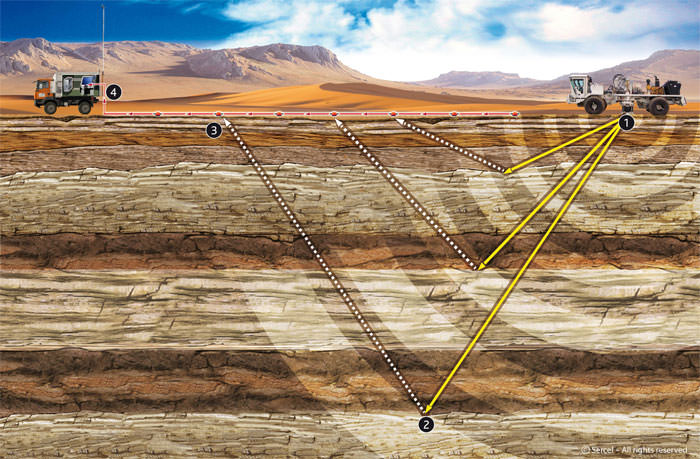
\includegraphics[width=12cm,height=6.5cm]{image/acquisition_terrestre.png}
  \end{figure}
    \onslide<2>
      \vspace{-0.3cm}
  \begin{figure}
   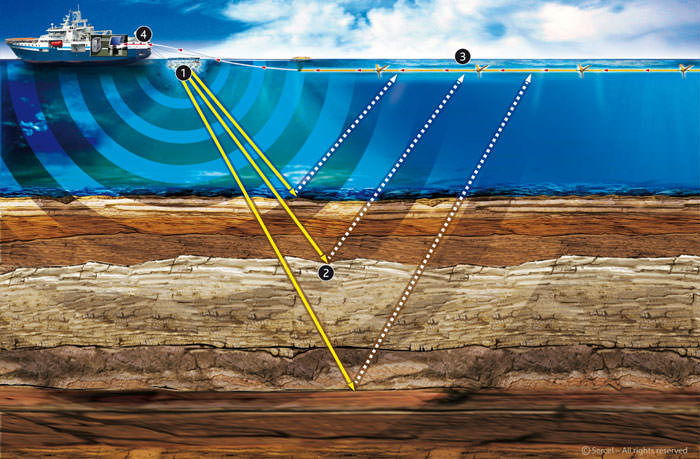
\includegraphics[width=12cm,height=6.5cm]{image/acquisition_marine.png}
  \end{figure}
  \end{overprint}

\end{frame}

\addtocounter{footnote}{-1}




% ============================================
% ====== Frame : Seismic Acquisition  ========
% ============================================
\begin{frame}{Seismic Acquisition}


  \begin{figure}
    \def\svgwidth{1.0\linewidth}
    \input{images/intro_1.pdf_tex}
  \end{figure}

\end{frame}

\begin{frame}[noframenumbering]{Seismic Acquisition}


  \begin{figure}
    \def\svgwidth{1.0\linewidth}
    \input{images/intro_2.pdf_tex}
  \end{figure}

\end{frame}

\newcommand\hideit[1]{%
  \only<0| handout:1>{\mbox{}}%
  \invisible<0| handout:1>{#1}}







% ============================================
% ====== Frame : FWI Workflow 1       ========
% ============================================
\subsection{FWI Workflow}

\begin{frame}{FWI Workflow}
\small
\vspace{-3.67cm}
\begin{columns}
\column{\dimexpr\paperwidth-10pt}
\begin{figure}
\def\svgwidth{1.0\linewidth}
\input{images/data.pdf_tex}
\end{figure}
\end{columns}
\end{frame}

\begin{frame}[noframenumbering]{FWI Workflow}
  \vspace{-0.5cm}
  \begin{columns}
    \column{\dimexpr\paperwidth-10pt}
    \begin{figure}
      \def\svgwidth{1.0\linewidth}
      \input{images/data_2.pdf_tex}
    \end{figure}
  \end{columns}
  \uncover<2->{
    \begin{equation}
      \CF(\model) = \frac{1}{2}||\textcolor{blue}{d_{obs}}-\textcolor{red}{\mathcal{F}(\model)}||^2
    \end{equation}
    \vspace{-0.2cm}
 \begin{itemize}
   \item $\mathcal{F}(m)$ is the restriction on the receivers of the simulated waves in the medium $\model$. (With $\model = \velocity, \density, \bulkmodulus$...)
   \item FWI: minimization problem by using adjoint state method \footcite{tarantolaInversionSeismicReflection1984} \footcite{laillySequenceStackMigrations1983}
 \end{itemize}

  }
\end{frame}

\addtocounter{footnote}{-2}






% ============================================
% ====== Frame : FWI Workflow 2       ========
% ============================================


\begin{frame}{FWI Workflow}
\begin{figure}
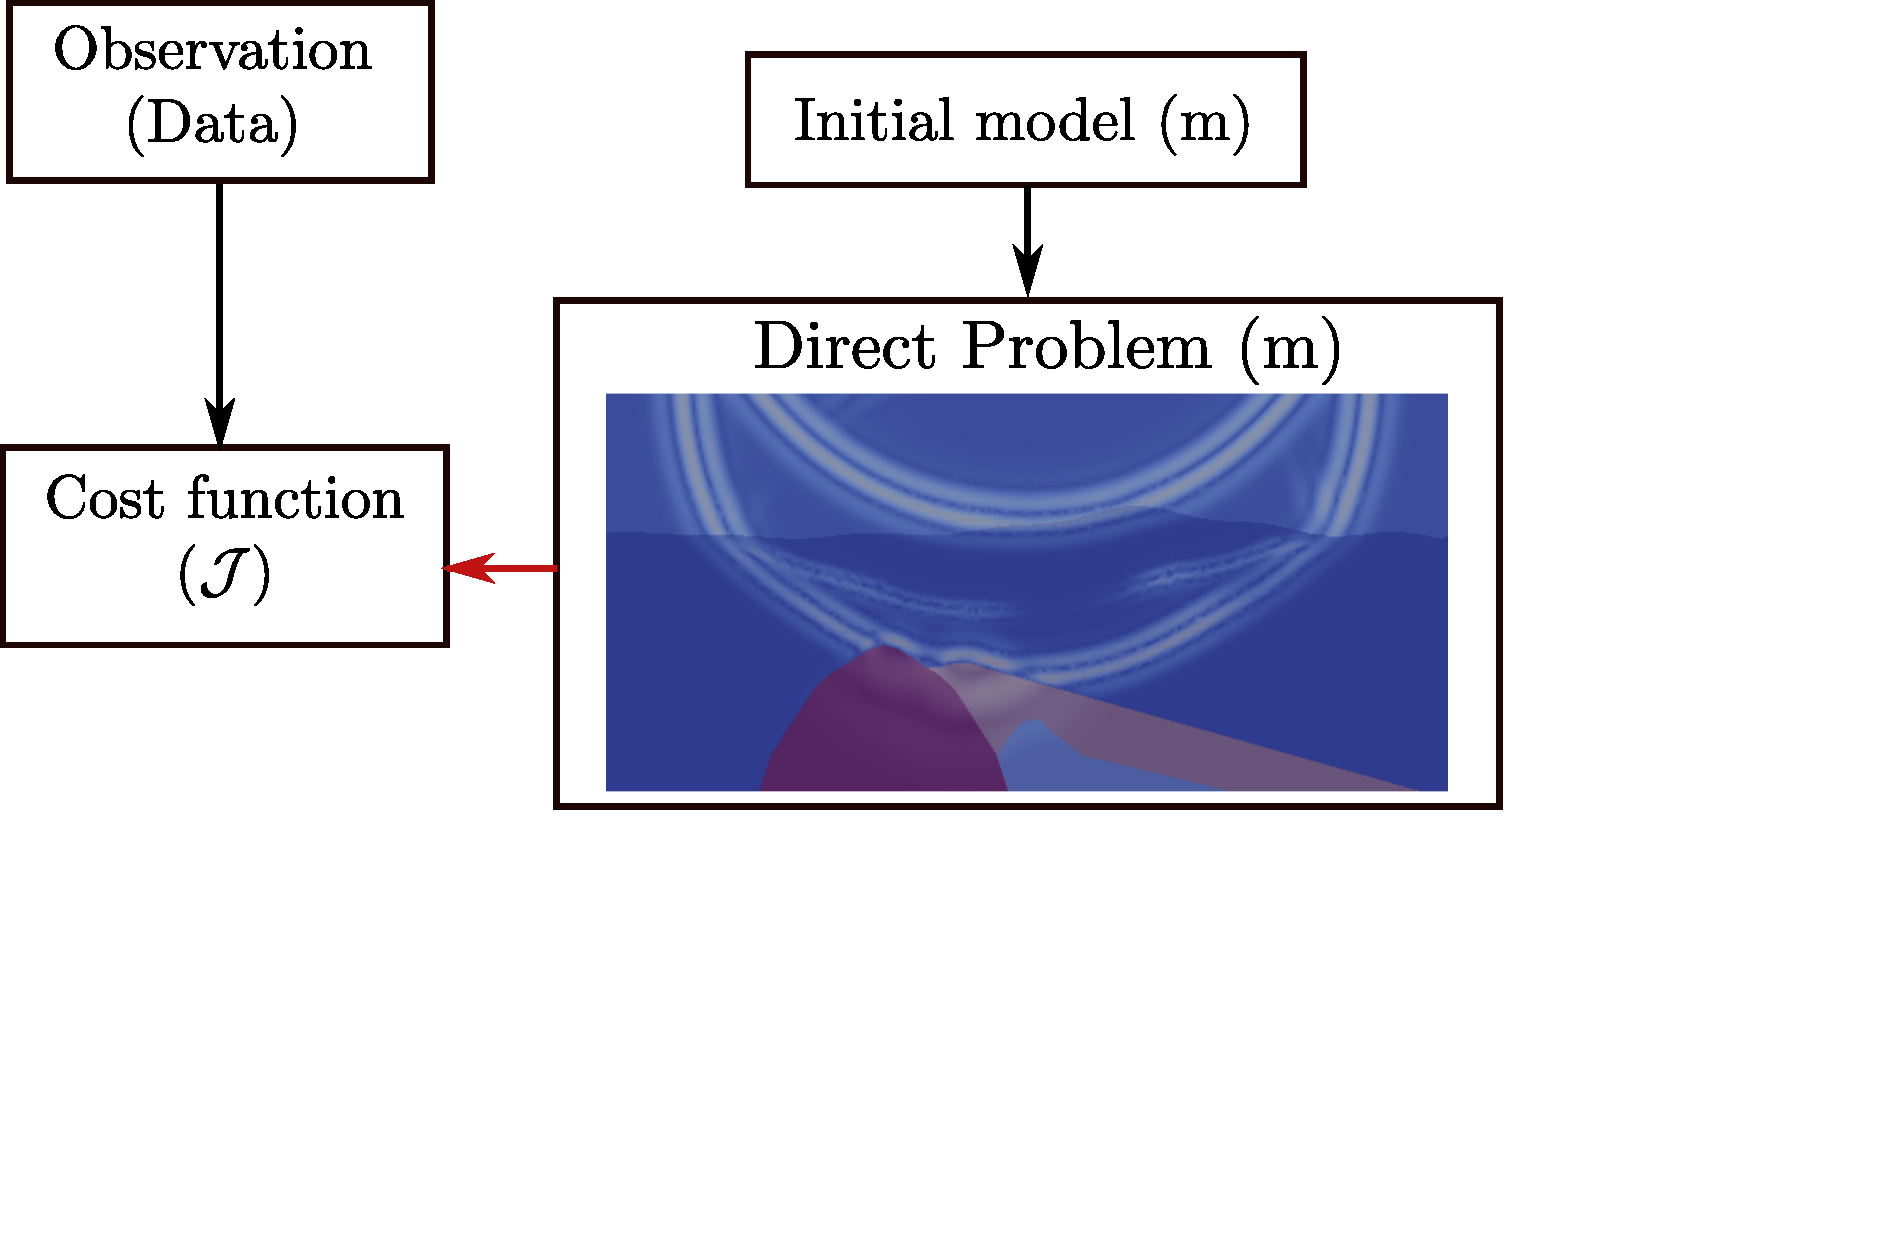
\includegraphics[scale=0.3]{image_inv_problem/pb_inv_workflow0.pdf}
\end{figure}
\end{frame}

\begin{frame}[noframenumbering]{FWI Workflow}
\begin{figure}
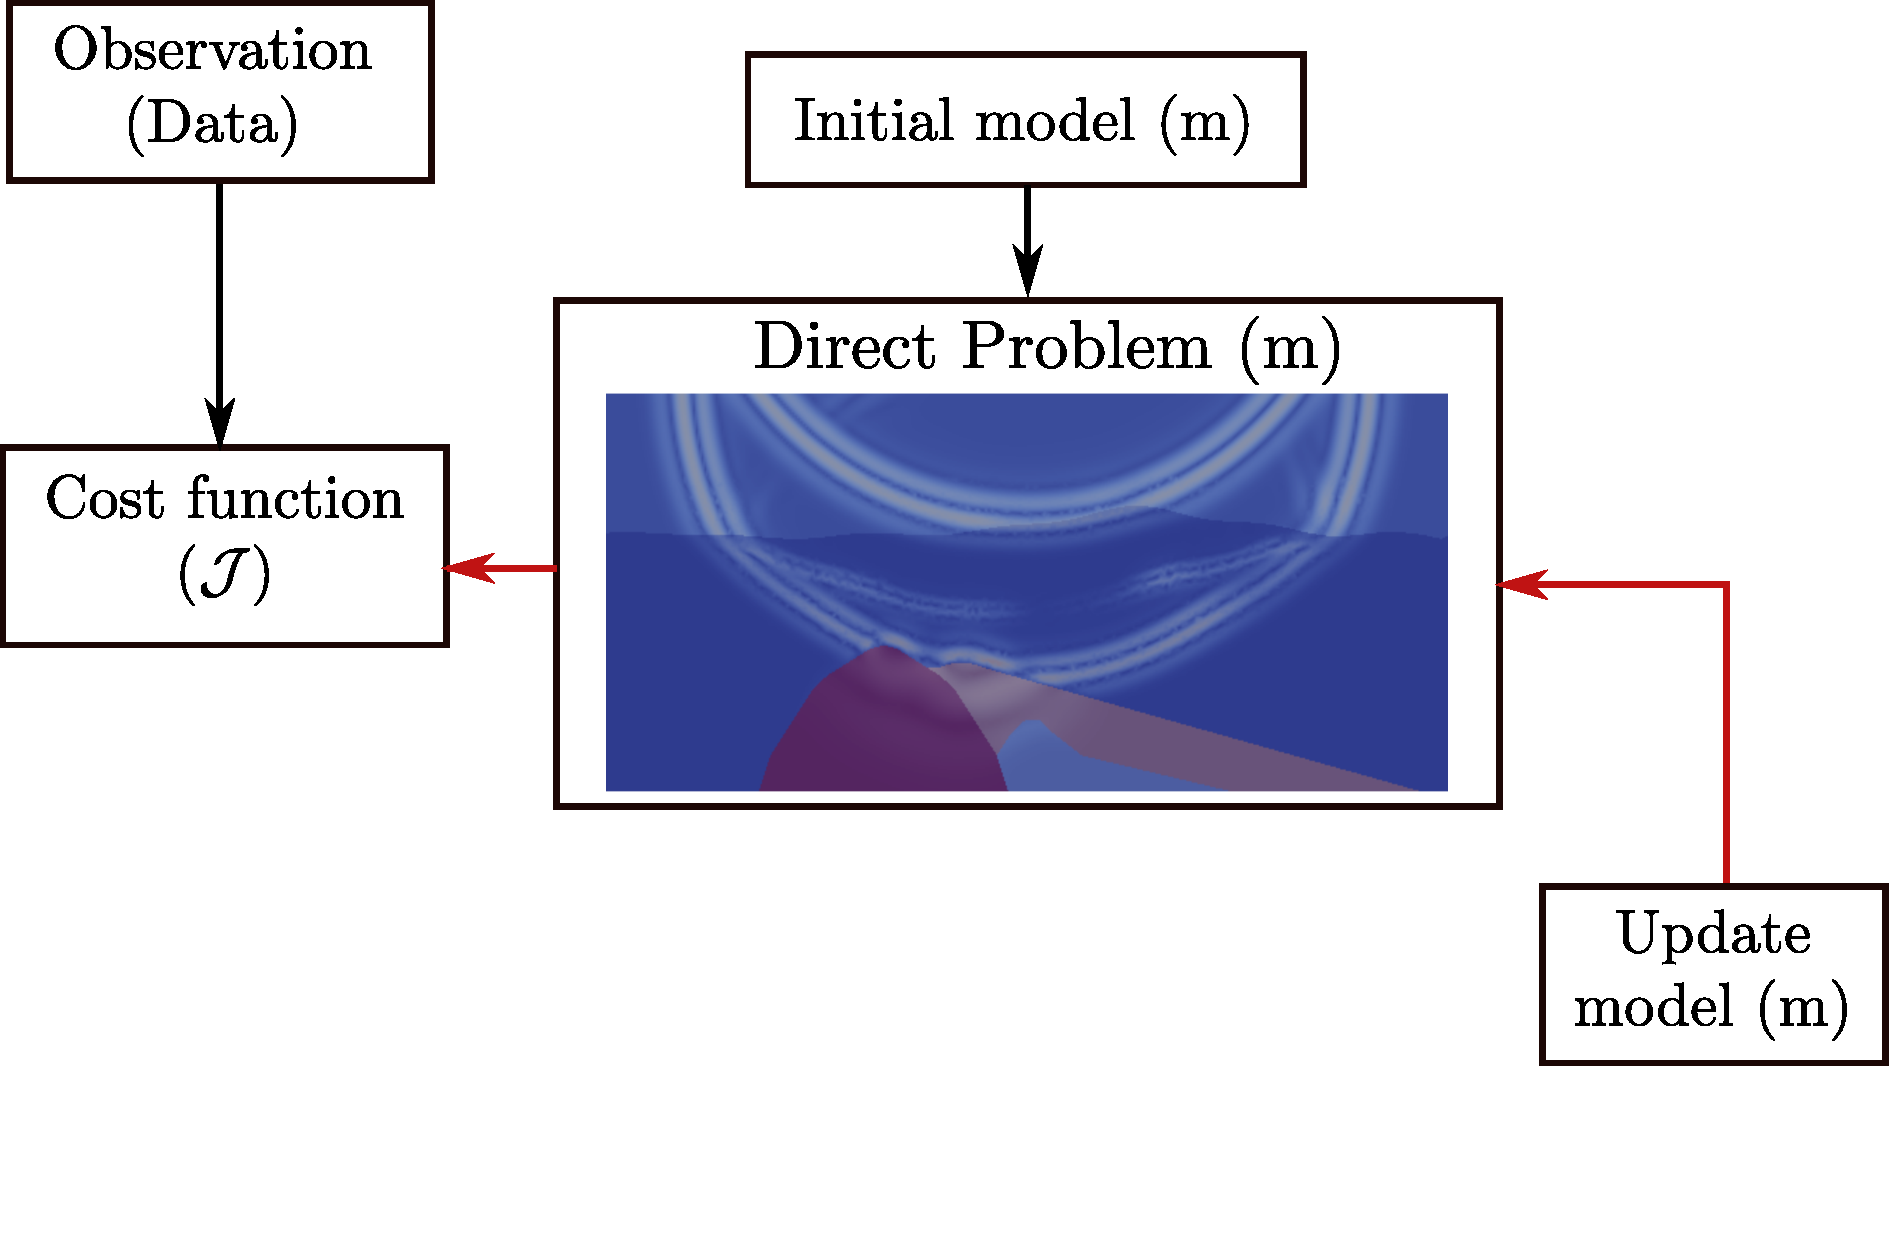
\includegraphics[scale=0.3]{image_inv_problem/pb_inv_workflow1.pdf}
\end{figure}
\end{frame}

\begin{frame}[noframenumbering]{FWI Workflow}
\begin{figure}
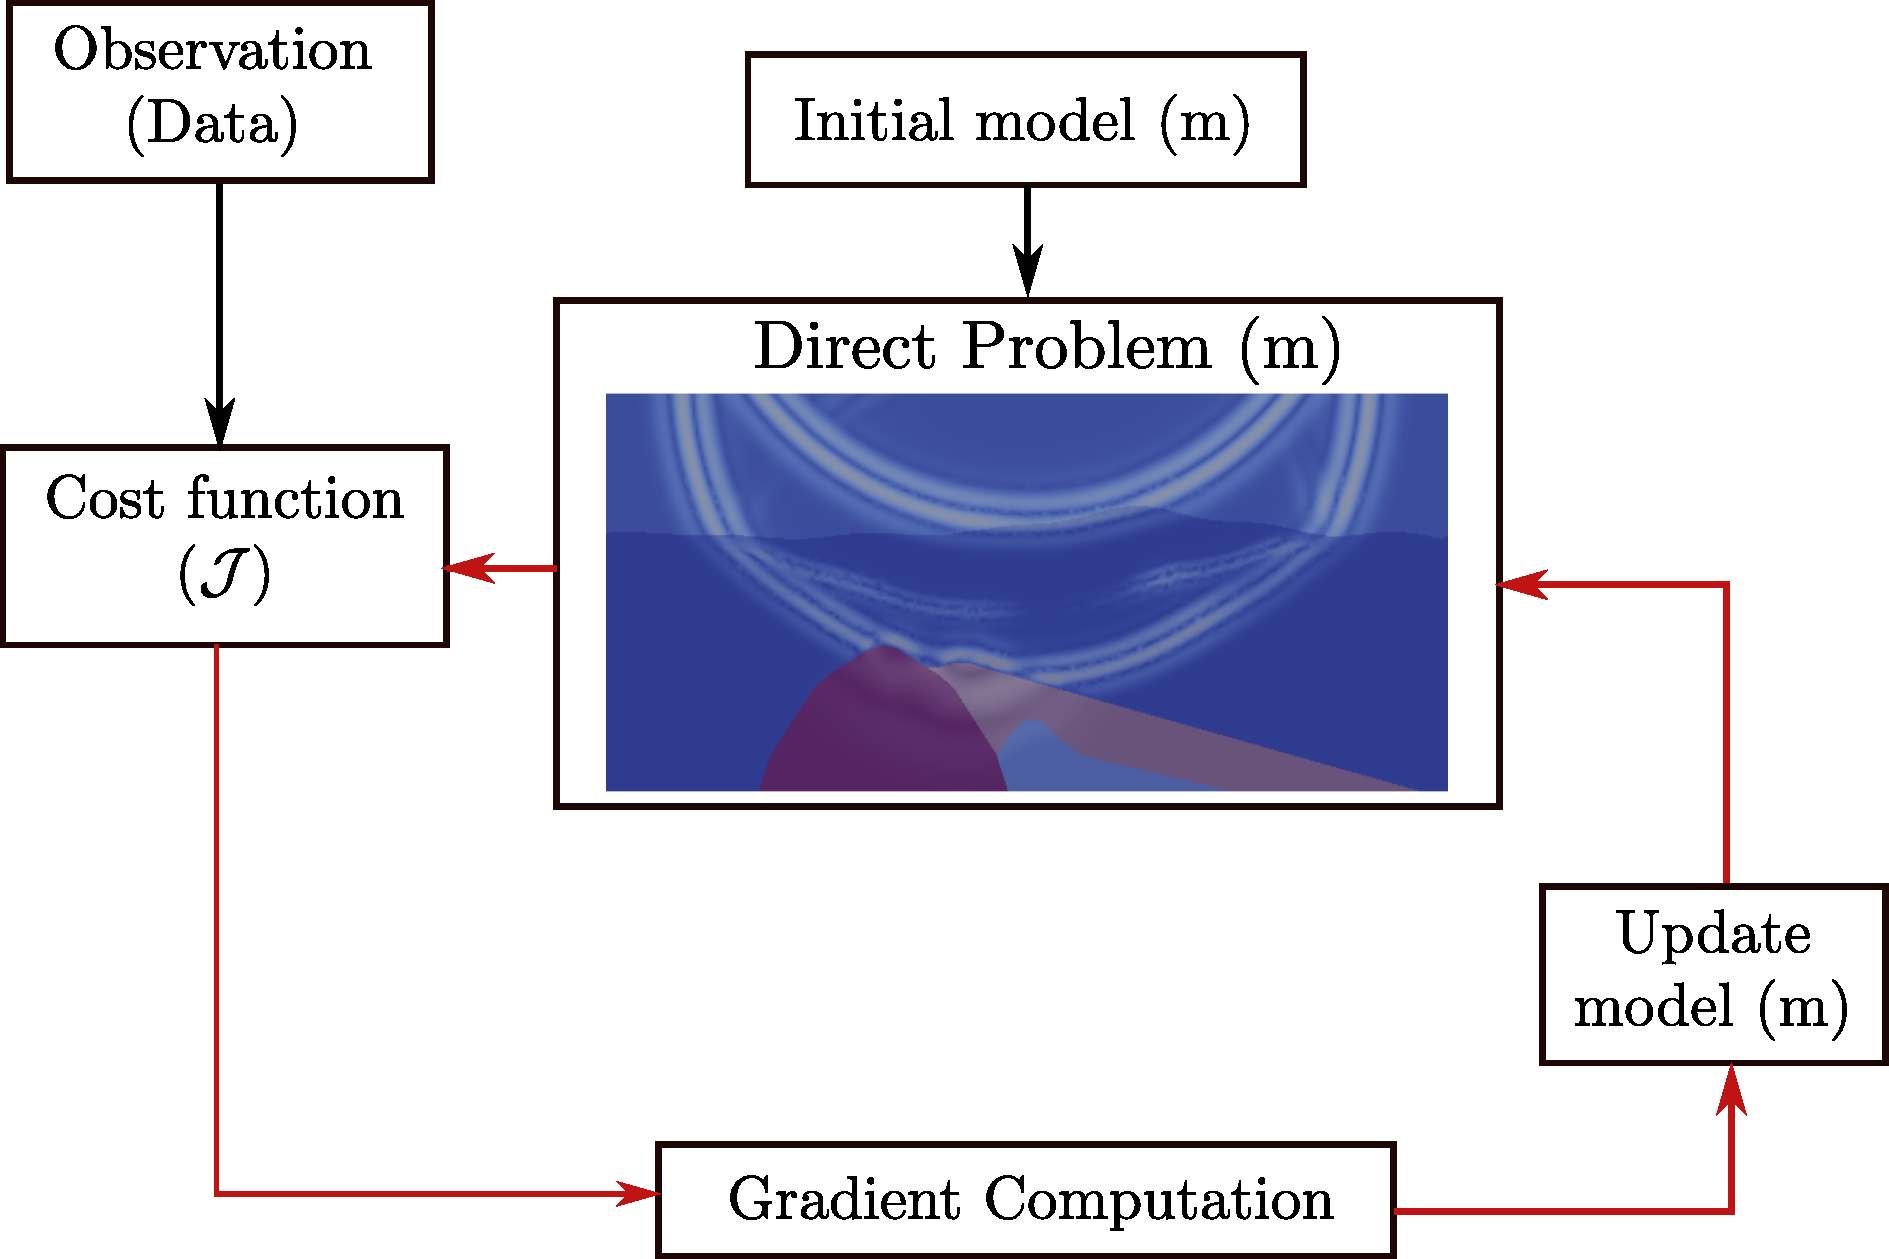
\includegraphics[scale=0.3]{image_inv_problem/pb_inv_workflow.pdf}
\end{figure}
\end{frame}

\begin{frame}[noframenumbering]{FWI Workflow}
\begin{figure}
  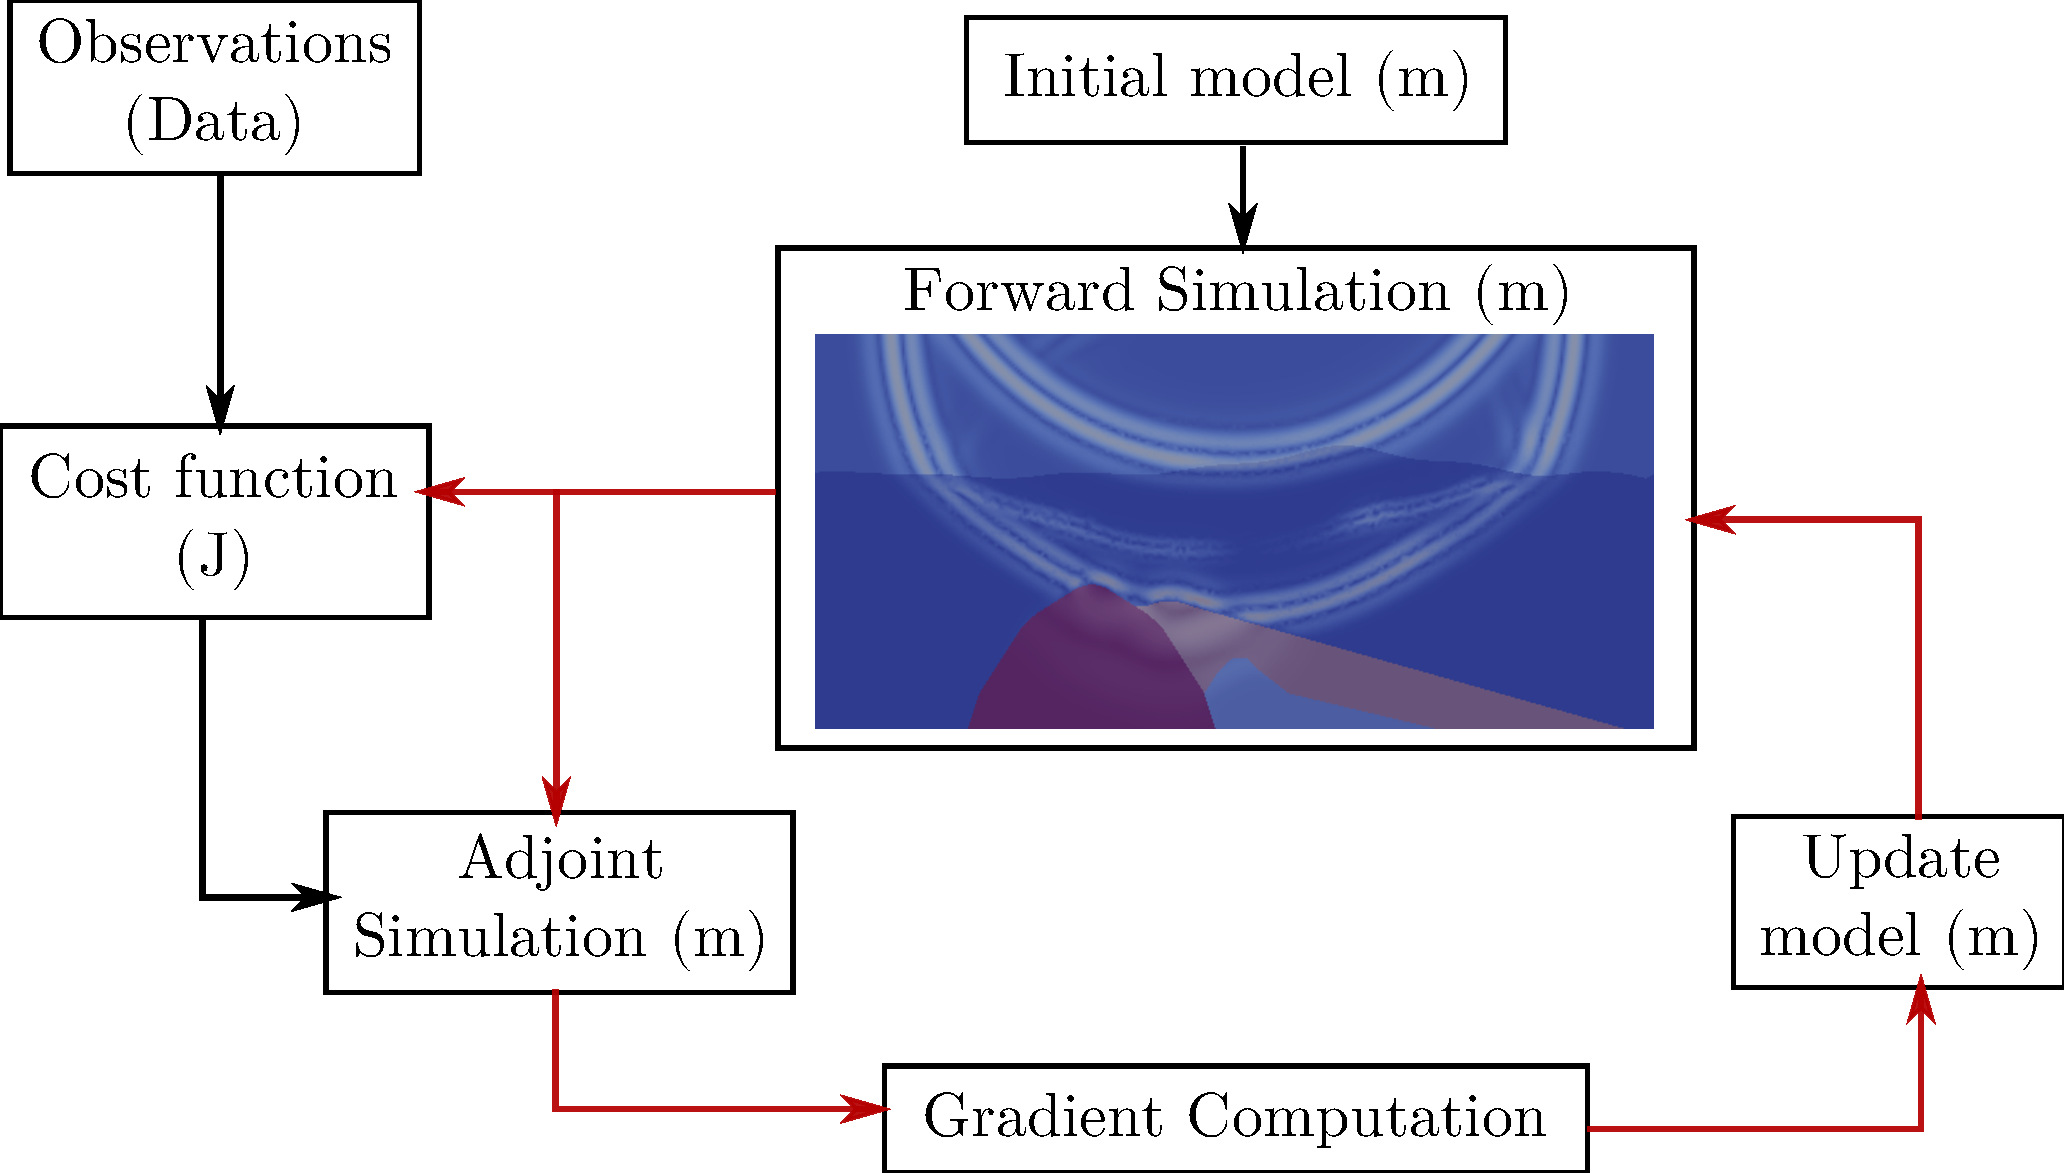
\includegraphics[scale=0.31]{fwi_test.pdf}
\end{figure}
\end{frame}

\begin{frame}[noframenumbering]{FWI Workflow}
\begin{figure}
  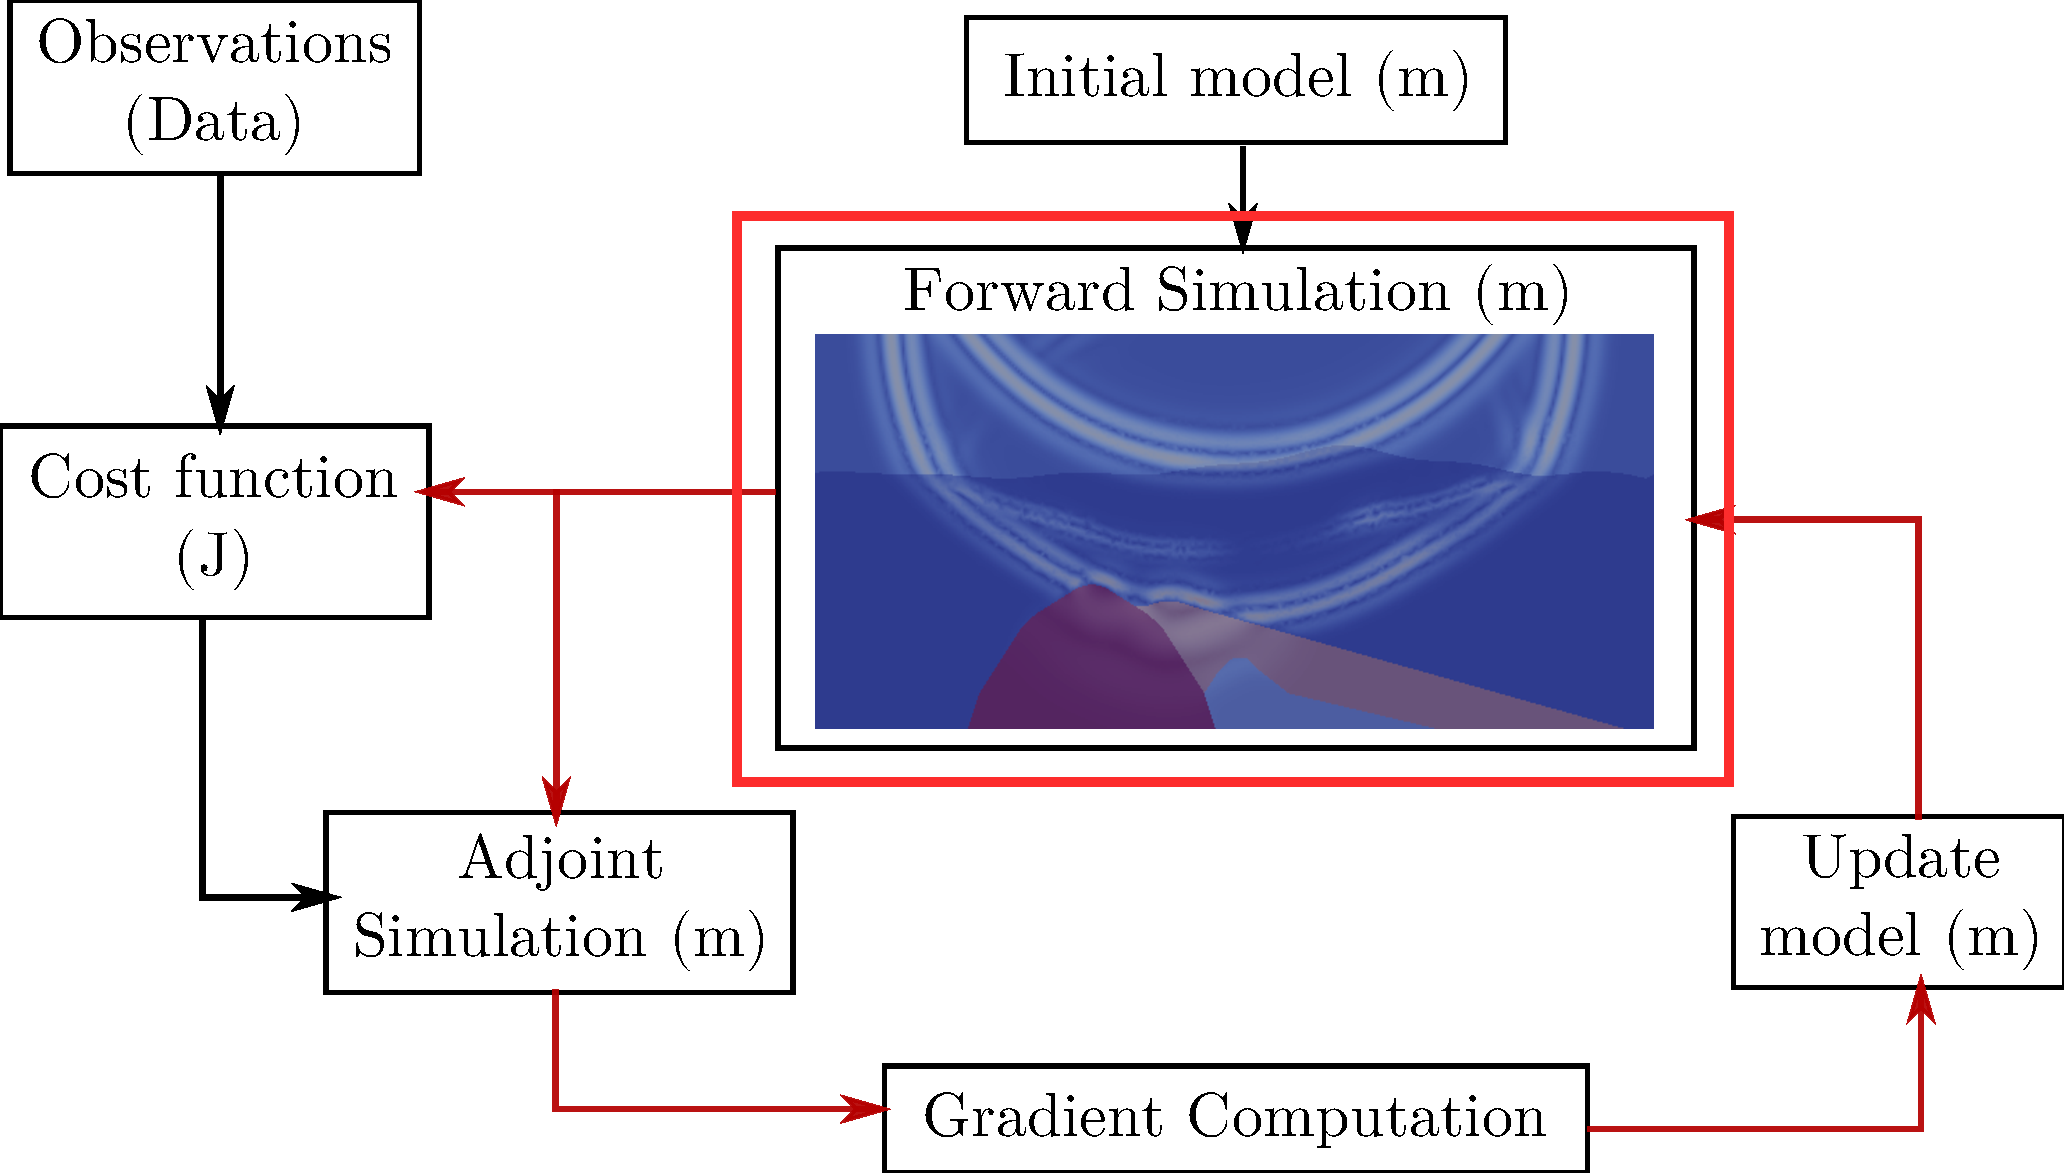
\includegraphics[scale=0.31]{fwi_test3.pdf}
\end{figure}
\end{frame}



% ============================================
% ====== Frame : Forward Continuous Model ====
% ============================================
{
  \AtBeginSection[]{}
}
\section{Forward Discretization}
\subsection{The continuous model}
\begin{frame}{Continuous Forward Model}
  \small
  First order acoustic wave equation:
  \vspace{-0.7cm}
  \begin{multicols}{2}
  \begin{empheq}[left=\empheqlbrace]{align}
    & \frac{1}{\density \velocity^2}\frac{\partial \contP}{\partial t}+\nabla \cdot \contV=f_p \text{~~ on $\boldsymbol{\Omega}$}\\
    & \density\frac{\partial \contV}{\partial t}+\nabla\contP=0  \text{~~ on $\boldsymbol{\Omega}$}\\
    & \contP=0 \text{~~ on $\textcolor{\myred}{\boldsymbol{\Gamma_1}}$} \\
    & \contP + \velocity \density \contV \cdot \normal=0 \text{~~ on $\textcolor{\myblue}{\boldsymbol{\Gamma_2}}$} \\
    & \contP(0) = 0 \text{, ~~~} \contV(0) = 0
  \end{empheq}

  \columnbreak

~ \\
\begin{center}
\renewcommand\tikzscale{1.0}
\begin{figure}[H]
\centering
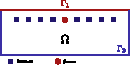
\includegraphics[scale=2.5]{image/truncated_domain.pdf}
\caption{Truncated infinite domain.} \label{truncated_domain}
\end{figure}
  \end{center}
  \end{multicols}

\vspace{-0.5cm}
\begin{block}{Variables:}

\begin{multicols}{2}

\begin{itemize}
\item $\contP$: the pressure (kg.m$^{-1}$.s$^{-2}$)
\item $\contV$: the wavespeed  (m.s$^{-1}$)
\end{itemize}

\columnbreak

\begin{itemize}
\item $\velocity$: velocity  (m.s$^{-1}$)
\item $\density$:  density  (kg.m$^{-3}$)
\item $\bm$:       bulk modulus ($\bm = \density  \velocity^2$) (kg.m$^{-1}$.s$^{-2}$)
\end{itemize}

\end{multicols}
\end{block}

\end{frame}

% ===================================================
% ====== Frame : Discontinuous Galerkin method ======
% ===================================================
\subsection{Discontinuous Galerkin method}
\begin{frame}{Discontinuous Galerkin method}
\vspace{-1.5cm}
Spatial discretization based on Discontinuous Galerkin methods:
\vspace{0.5cm}
\begin{itemize}
\item<1-> Approximation made with discontinuous basis functions
\item<2-> Based on unstructured triangles and unstructured tetrahedra
\item<3-> Natural $hp$-adaptivity
\item<4-> Block diagonal mass matrix
\item<5-> High scalability of the solver \footcite{shraggeSolving3DAcoustic2014} (suitable for HPC environnement)
\end{itemize}

\begin{overprint}
\onslide<3>
 \begin{multicols}{2}
   \begin{figure}[H]
     \centering
     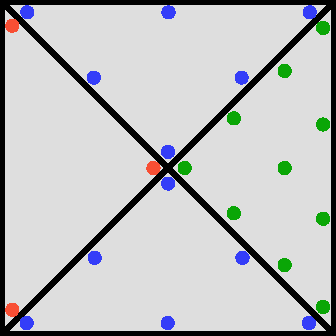
\includegraphics[scale=0.3]{image/p_adaptivity.pdf}
     \caption*{Illustration of \\ $p$-adaptivity.}
     \label{p_adapt_sketch}
   \end{figure}
   \columnbreak
   \begin{figure}[H]
     \centering
     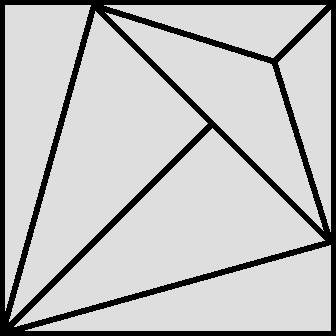
\includegraphics[scale=0.3]{image/h_adaptivity.pdf}
     \caption*{Illustration of \\ $h$-adaptivity.}
     \label{h_adapt_sketch}
   \end{figure}
 \end{multicols}

\onslide<4->

\scriptsize
  \begin{empheq}[left=\empheqlbrace]{align}
  & \frac{1}{\bm} \Mass^\element  \frac{\partial \textcolor{\myred}{\coefPolP}^\element}{\partial t}
  + \sum_{d=1}^\dim \Stiff_\xd^\element \textcolor{\myred}{\coefPolVd}^\element
  + \sum_{\Edge} \Mass_\Edge^\element \FluxP^\Edge(\textcolor{\myred}{\coefPolP},\textcolor{\myred}{\coefPolV})
  = \frac{1}{\bm} \Mass^\element \coefpolSource^\element, \\
  & \density \Mass^\element  \frac{\partial \textcolor{\myred}{\coefPolV_d}^\element}{\partial t}
  + \Stiff_\xd^\element \textcolor{\myred}{\coefPolP}^\element + \sum_\Edge \Mass_\Edge \FluxV_d^\Edge (\textcolor{\myred}{\coefPolP},\textcolor{\myred}{\coefPolV})
  = 0  \qquad\text{(for $d=1\,\,\text{to}\,\,\dim$)} \,,
  \label{local_semi_disc2}
  \end{empheq}
\end{overprint}
\vspace{-5cm}

\end{frame}

% ===================================================
% ====== Frame : Speed up studies ===================
% ===================================================

\setbeamercovered{invisible}
\begin{frame}{Scalability Study}{Comparison DG / FD}
\small
Speed up comparison on a 5s simulation in 3D (9km $\times$ 5km $\times$ 3km):

\setlength{\plotwidth}{7cm}
\setlength{\plotheight}{3.7cm}
\begin{figure}[!htbp]
\centering
    \begin{tikzpicture}
      \begin{axis}[%
          width=\plotwidth, height=\plotheight,,
          at={(0,0)},scale only axis,separate axis lines,
          xlabel={\scriptsize{Number of CPU}},
          ylabel={\scriptsize{Speed-up}},
          xmin=1,xmax=768,
%          ymin=0,ymax=1,
          legend pos= north west
          %ymin=0.98,ymax=1.22
        ]
        \addplot[color=black,mark options={solid}, mark=triangle*,
        line width=1.5pt,
        mark size=0pt]
        table[x=monx,y=mony]
        {graph/ideal_speed_up.txt};
        \addlegendentry{\scriptsize{Ideal Speed-up}}
        \addplot[color=blue!80!black,mark options={solid}, mark=triangle*,smooth,
        line width=1pt,
        mark size=0pt]
        table[x=monx,y=mony]
        {graph/dg_speed_up_pres.txt};
        \addlegendentry{\scriptsize{DG}}
        \addplot[color=red,mark options={solid}, mark=*,
        line width=0.8pt,
        mark size=0pt]
        table[x=monx,y=mony]
        {graph/df_speed_up_pres.txt};
        \addlegendentry{\scriptsize{FD}}
\end{axis}
\end{tikzpicture}
\end{figure}

\vspace{-0.2cm}
\uncover<2->{
\begin{block}{\danger Warning}
\small This is an example to illustrate the DG HPC properties. \\
Further comparisons are required to properly compare the two methods.
\end{block}
}

\end{frame}




% ===================================================
% ====== Frame : Time domain motivation =============
% ===================================================
\subsection{Time-Domain}
\begin{frame}{Time-Domain Motivations}

\begin{itemize}
\item<2-> Frequency domain are limited by the ability of solver to solve large-scale problems \footcite{operto20073d}.
\item<3-> Explicit time-schemes do not require the inversion of large size matrices.
\item<4-> In time domain, intermediate results can be stored on the disk to reduce the memory burden (for gradient computation).
\item<5-> In case of disk storage limitation , checkpointing\footcite{griewankAchievingLogarithmicGrowth1992} strategies exists to reduce the overall storage cost.
\end{itemize}

\end{frame}


% ===================================================
% ====== Frame : Time schemes =======================
% ===================================================

\begin{frame}{Time-schemes}
\scriptsize
Three explicit time-schemes as been studied: \\
\begin{multicols}{3}
\textbf{Runge-Kutta 2}

\columnbreak

\textbf{Runge-Kutta 4}

\columnbreak

\textbf{Adams Bashforth 3}
\end{multicols}

\begin{block}{CFL condition\footnotemark}
Initially, the time step $\deltat$ was not computed in the solver.

\begin{multicols}{2}
\begin{equation}
\deltat = \underset{\elementK}{\min}(\deltat^\elementK)\,,
\end{equation}
\begin{equation}
        \deltat^\elementK \le C \frac{r^\elementK}{\velocity^\elementK p^\elementK}\,.
\end{equation}
\vfill

\columnbreak
\tiny
Where:
\begin{itemize}
\item $C$: the CFL condition;
\item $r^\elementK$: the inner radius of the cell $\elementK$;
\item $\velocity^\elementK$: the wavespeed parameter associated to $\elementK$;
\item $p^\elementK$: the polynomial order of approximation in $\elementK$.
\end{itemize}
\end{multicols}
\end{block}
\footcitetext{hesthavenNodalDiscontinuousGalerkin2007}
\end{frame}


\begin{frame}[noframenumbering]{Time-schemes}
\scriptsize
Three explicit time-schemes as been studied: \\
\begin{multicols}{3}
\textbf{Runge-Kutta 2}

\columnbreak

\textbf{Runge-Kutta 4}

\columnbreak

\textbf{Adams Bashforth 3}
\end{multicols}

\begin{block}{CFL condition}
Initially, the time step $\deltat$ was not computed in the solver.

\begin{multicols}{2}
\begin{equation}
\deltat = \underset{\elementK}{\min}(\deltat^\elementK)\,,
\end{equation}
\begin{equation}
        \deltat^\elementK \le C \frac{r^\elementK}{\velocity^\elementK p^\elementK}\,.
\end{equation}
\vfill

\columnbreak
\tiny
Where:
\begin{itemize}
\item $C$: the CFL condition;
\item $r^\elementK$: the inner radius of the cell $\elementK$;
\item $\velocity^\elementK$: the wavespeed parameter associated to $\elementK$;
\item $p^\elementK$: the polynomial order of approximation in $\elementK$.
\end{itemize}
\end{multicols}
\end{block}
\begin{overprint}
\onslide<1>
\begin{figure}[H]
\centering
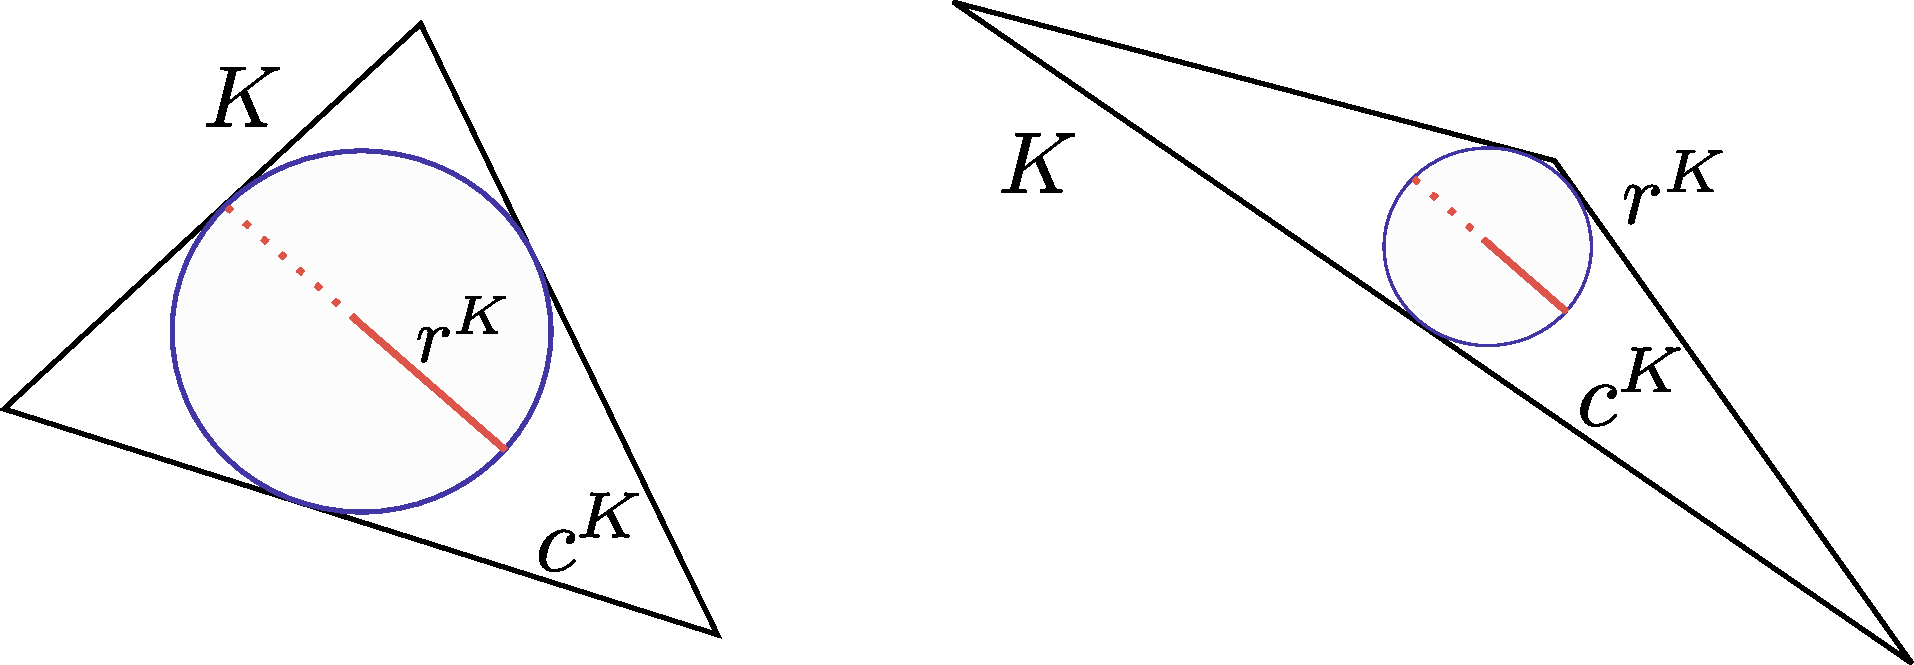
\includegraphics[scale=0.2]{image/cfl.pdf}
\label{cfl_sketch}
\end{figure}
\onslide<2>
\begin{table}[H]
\centering
\begin{tabular}{|l|l|l|l|}
\hline
  & RK2  & RK4  & AB3  \\ \hline
C & 0.66 & 0.84 & 0.18 \\ \hline
\end{tabular}
\caption{CFL coefficients for different time schemes.}
\label{coef_cfl}
\end{table}
\end{overprint}

\end{frame}



\subsection{Bernstein-Bézier}
 \begin{frame}{Polynomial bases}
 \scriptsize
 Two polynomial basis has been studied:
 \begin{multicols}{2}
 \textbf{Lagrange} (Nodal)

\vspace{0.5cm}
\begin{figure}[H]
\centering
\setlength{\plotwidth}{3.5cm}
\setlength{\plotheight}{2.5cm}
    \begin{tikzpicture}
      \begin{axis}[%
          width=\plotwidth, height=\plotheight,,
          at={(0,0)},scale only axis,separate axis lines,
          xlabel={$x$},
          %%   ymode=log,
          %yminorticks=true,
           xmin=0,xmax=1,
           %ymin=0,ymax=1,
          legend pos=outer north east
          %ymin=0.98,ymax=1.22
        ]

        %% load current data
        %% -----------------
        \addplot[color=blue!50!black,mark options={solid}, mark=triangle*,
          line width=2pt,
          mark size=0pt]
        table[x=x,y=1]
        {graph/lagrange_5.dat};
        \addlegendentry{$\ell_1^5$}

 \addplot[color=red!75!black,mark options={solid}, mark=*,
          line width=2pt,
          mark size=0pt]
        table[x=x,y=2]
        {graph/lagrange_5.dat};
        \addlegendentry{$\ell_2^5$}

 \addplot[color=green!50!black,mark options={solid}, mark=square*,
          line width=2pt,
          mark size=0pt]
        table[x=x,y=3]
        {graph/lagrange_5.dat};
        \addlegendentry{$\ell_3^5$}

 \addplot[color=yellow!80!black,mark options={solid}, mark=square*,
          line width=2pt,
          mark size=0pt]
        table[x=x,y=4]
        {graph/lagrange_5.dat};
        \addlegendentry{$\ell_4^5$}

 \addplot[color=green!75!white,mark options={solid}, mark=square*,
          line width=2pt,
          mark size=0pt]
        table[x=x,y=5]
        {graph/lagrange_5.dat};
        \addlegendentry{$\ell_5^5$}

 \addplot[color=blue!40!white,mark options={solid}, mark=diamond*,
          line width=2pt,
          mark size=0pt]
        table[x=x,y=6]
        {graph/lagrange_5.dat};
        \addlegendentry{$\ell_6^5$}
      \end{axis}
      %% --------------------------------------------------------------------
    \end{tikzpicture}

\caption{\scriptsize{Illustration of $P^5([0,1])$ Lagrange basis.}}
\label{lagrange_5}
\end{figure}

\columnbreak
\textbf{Bernstein-Bézier \footcite{chanGPUacceleratedBernsteinBezierDiscontinuous2016}} (Modal)

\begin{figure}[H]
\centering
\setlength{\plotwidth}{3.5cm}
\setlength{\plotheight}{2.5cm}
    \begin{tikzpicture}
      \begin{axis}[%
          width=\plotwidth, height=\plotheight,,
          at={(0,0)},scale only axis,separate axis lines,
          xlabel={$\xx$},
          %%   ymode=log,
          %yminorticks=true,
           xmin=0,xmax=1,
           ymin=0,ymax=1,
          legend pos=outer north east
          %ymin=0.98,ymax=1.22
        ]

        %% load current data
        %% -----------------
        \addplot[color=blue!50!black,mark options={solid}, mark=triangle*,
          line width=2pt,
          mark size=0pt]
        table[x=x,y=50]
        {graph/bb_5.dat};
        \addlegendentry{$B^5_{5,0}$}

 \addplot[color=red!75!black,mark options={solid}, mark=*,
          line width=2pt,
          mark size=0pt]
        table[x=x,y=41]
        {graph/bb_5.dat};
        \addlegendentry{$B^5_{4,1}$}

 \addplot[color=green!50!black,mark options={solid}, mark=square*,
          line width=2pt,
          mark size=0pt]
        table[x=x,y=32]
        {graph/bb_5.dat};
        \addlegendentry{$B^5_{3,2}$}

 \addplot[color=yellow!80!black,mark options={solid}, mark=square*,
          line width=2pt,
          mark size=0pt]
        table[x=x,y=23]
        {graph/bb_5.dat};
        \addlegendentry{$B^5_{2,3}$}

 \addplot[color=green!75!white,mark options={solid}, mark=square*,
          line width=2pt,
          mark size=0pt]
        table[x=x,y=14]
        {graph/bb_5.dat};
        \addlegendentry{$B^5_{1,4}$}

 \addplot[color=blue!40!white,mark options={solid}, mark=diamond*,
          line width=2pt,
          mark size=0pt]
        table[x=x,y=05]
        {graph/bb_5.dat};
        \addlegendentry{$B^5_{0,5}$}
      \end{axis}
      %% --------------------------------------------------------------------
    \end{tikzpicture}

\caption{\scriptsize{Illustration of $P^5([0,1])$ Bernstein-Bézier basis.}}
\label{bb_base_5}
\end{figure}

\end{multicols}

\uncover<2->{
  \begin{tikzpicture}[remember picture,overlay]
    \draw [red,ultra thick,rounded corners] (0,0) rectangle (6.2,6.5);
  \end{tikzpicture}
}
\end{frame}


\begin{frame}{Bernstein-Bézier polynomial basis}
\vspace{-0.2cm}
\scriptsize
\begin{block}{\scriptsize{Polynomial basis expression:}}
In an arbitrary dimension, $\balpha \in \mathbb{N}^{\dim+1}$ with $\sum_{i=0}^N \alpha_i = N$
and $\blambda \in [0,1]^{\dim+1}$ with $\sum_{i=0}^N \hat{\lambda}_i = 1$.
For example, we have in 3D the following notation:
\begin{equation}
        B^\PolOrder_\balpha(\blambda) = B^\PolOrder_{ijkl}(\lzero,\lone,\ltwo,\lthree) = C^\PolOrder_{ijkl} \lzero^i \lone^j \ltwo^k \lthree^l = \frac{\PolOrder!}{i!j!k!l!}\lzero^i \lone^j \ltwo^k \lthree^l
\end{equation}
\end{block}
\vspace{-0.1cm}
\uncover<2->{
\begin{block}{\scriptsize{Property 1: Sparse elevation order}}
A Bernstein polynomial of order $N-1$
can be represented with a linear combination of $\dim+1$ Bernstein polynomials
of order $\PolOrder$ as follows:

\begin{equation}
B^{\PolOrder-1}_\balpha(\blambda) = \sum_{i=0}^\dim \frac{\alpha_i+1}{\PolOrder} B^\PolOrder_{\balpha + \ecan_i}(\blambda)\,. \label{elev_order_bb}
\end{equation}
\end{block}
}
\vspace{-0.1cm}
\uncover<3->{
\begin{block}{\scriptsize{Property 2: Sparse dervative operator}}
The derivative of a Bernstein polynomial $B^\PolOrder_\balpha$ with respect to $\hat{\lambda}_i$ is given by:
\begin{equation}
\frac{\partial B^\PolOrder_\balpha}{\partial \hat{\lambda}_i} (\blambda)= N B^{\PolOrder-1}_{\balpha-\ecan_i} (\blambda)\,.
\end{equation}
\end{block}
}
\end{frame}


\begin{frame}{Results using Bernstein-Bézier polynomial basis:}

\begin{figure}[htbp]
\begin{subfigure}{0.45\textwidth}
\centering
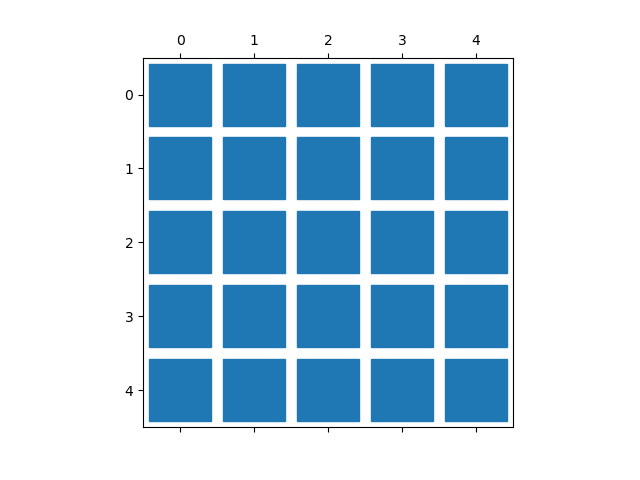
\includegraphics[scale=0.2]{image/dx_lag_4.png}
\caption{$\Diffx$ for Lagrange and $\PolOrder=4$.}
\end{subfigure}
\begin{subfigure}{0.45\textwidth}
\centering
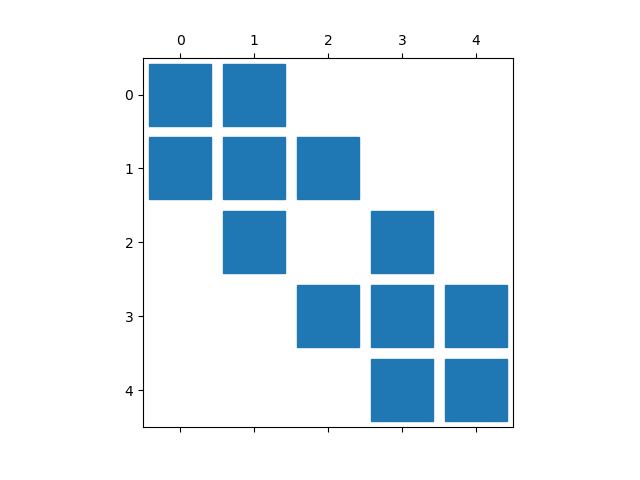
\includegraphics[scale=0.2]{image/dx_bb_4.png}
\caption{$\Diffx$ for Bernstein and $\PolOrder=4$.}
\end{subfigure}
\begin{subfigure}{0.45\textwidth}
\centering
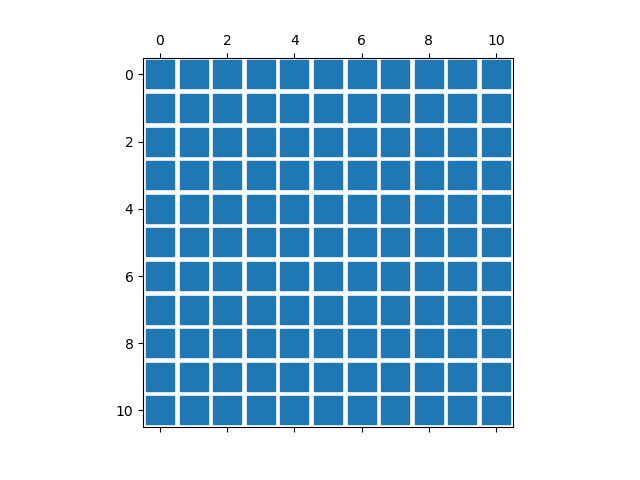
\includegraphics[scale=0.2]{image/dx_lag_10.png}
\caption{$\Diffx$ for Lagrange and $\PolOrder=10$.}
\end{subfigure}
\begin{subfigure}{0.45\textwidth}
\centering
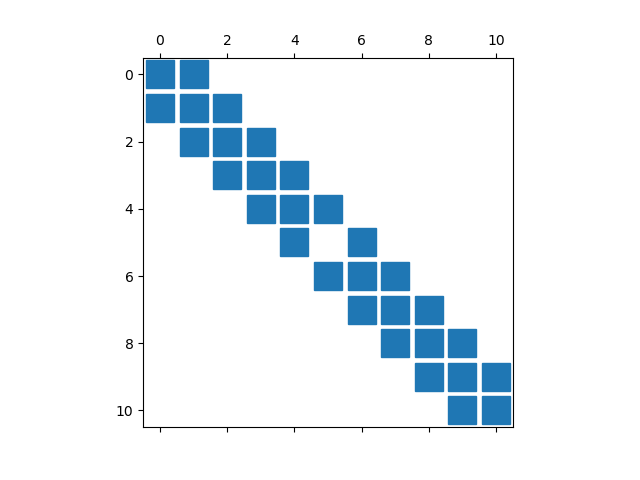
\includegraphics[scale=0.2]{image/dx_bb_10.png}
\caption{$\Diffx$ for Bernstein and $\PolOrder=10$.}
\end{subfigure}
\caption{Sparsity comparison between Lagrange and Bernstein
$\Diffx$ operator ($\Diffx =  \MassRef^{-1} \StiffRef_\refxx$).}
\label{dx_sparse_pattern}
\end{figure}
\end{frame}

\begin{frame}[noframenumbering]{Results using Bernstein-Bézier polynomial basis:}
\setlength{\plotwidth}{6.0cm}
\setlength{\plotheight}{4.5cm}
\begin{figure}[htbp]
\centering
  %% \begin{subfigure}[b]{0.5\textwidth}
    \begin{tikzpicture}
      \begin{axis}[%
          width=\plotwidth, height=\plotheight,,
          at={(0,0)},scale only axis,separate axis lines,xminorticks=true,
          xlabel={Polynomial order $\PolOrder$},
          ylabel={NZV},
          xmin=0,xmax=21,
          legend pos=north west
        ]
        %% load current data
        %% -----------------
        \addplot[color=blue!50!black,mark options={solid}, mark = triangle,
          line width=1pt,
          mark size=2pt]
        table[x=order,y=nzv]
        {graph/Bernstein_sparse.txt};
        \addlegendentry{Bernstein-Bézier}
        \addplot[color=red!50!black,mark options={solid}, mark = *,
          line width=1pt,
          mark size=2pt]
        table[x=order,y=nzv]
        {graph/Lagrange_sparse.txt};
        \addlegendentry{Lagrange}
        %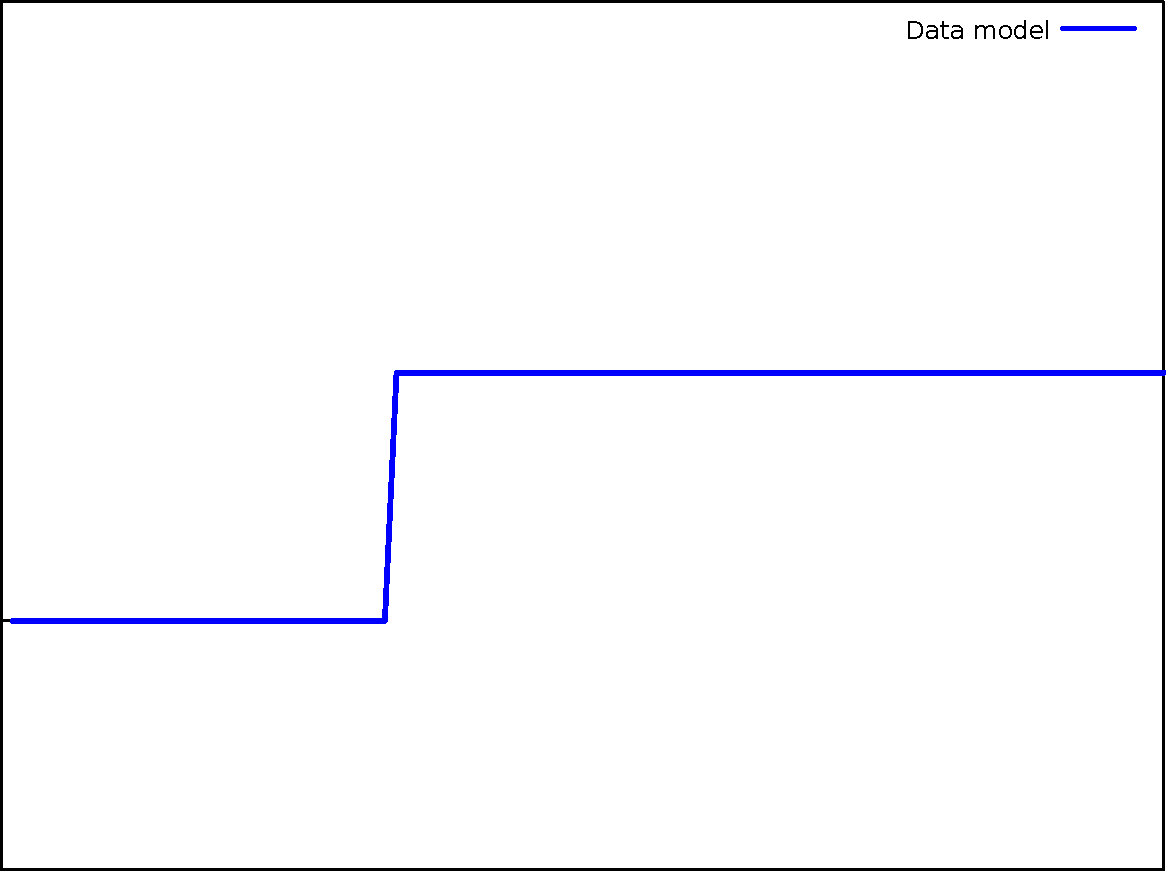
\includegraphics{images/data_bis.pdf}
      \end{axis}
      %% --------------------------------------------------------------------
    \end{tikzpicture}
  %%   \caption{}
  %%   \label{nzv_order}
  %% \end{subfigure}
  %% \begin{subfigure}[b]{0.5\textwidth}
  %%   \setlength{\plotwidth}{6.0cm}
  %%   \setlength{\plotheight}{4.5cm}
  %%   \begin{tikzpicture}
  %%     \begin{axis}[%
  %%         width=\plotwidth, height=\plotheight,,
  %%         at={(0,0)},scale only axis,separate axis lines,xminorticks=true,
  %%         xlabel={Polynomial order $\PolOrder$},
  %%         ylabel={Ratio},
  %%         %%   ymode=log,
  %%         %yminorticks=true,
  %%         xmin=0,xmax=21,
  %%         legend pos=north east
  %%         %ymin=0.98,ymax=1.22
  %%       ]

  %%       %% load current data
  %%       %% -----------------
  %%       \addplot[color=blue!50!black,mark options={solid}, mark = triangle,
  %%         line width=1pt,
  %%         mark size=2pt]
  %%       table[x=order,y=ratio]
  %%       {graph/Bernstein_sparse.txt};
  %%       \addlegendentry{Bernstein-Bézier}
  %%       \addplot[color=red!50!black,mark options={solid}, mark = *,
  %%         line width=1pt,
  %%         mark size=2pt]
  %%       table[x=order,y=ratio]
  %%       {graph/Lagrange_sparse.txt};
  %%       \addlegendentry{Lagrange}
  %%       %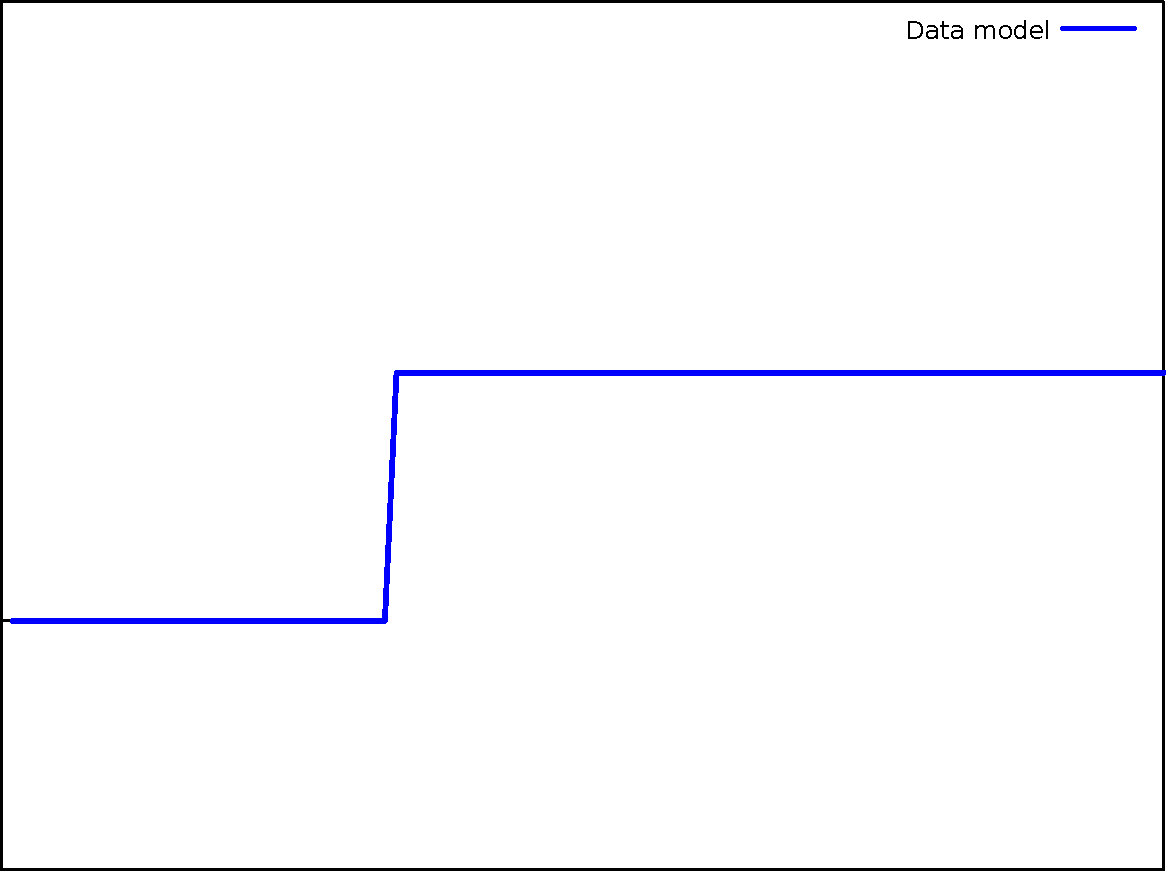
\includegraphics{images/data_bis.pdf}
  %%     \end{axis}
  %%     %% --------------------------------------------------------------------
  %%   \end{tikzpicture}
  %%   \caption{}
  %%   \label{ratio_order}
  %% \end{subfigure}

  \caption{Non zero values (NZV) of the global volume operator as a function of the polynomial order.}
  \label{bb_lag_comp_1d}
\end{figure}

\end{frame}



\begin{frame}[noframenumbering]{Results using Bernstein-Bézier polynomial basis:}
\scriptsize
\vspace{0.5cm}
\begin{table}[H]
    \centering
    \begin{tabular}{|l|l|l|l|l|l|}
    \hline
        \textbf{Sigsbee (2D)} & P1 & P2 & P3 & P4 & P5 \\ \hline
        Number of elements ($\nbelem$) & 569522 & 243636 & 121235 & 66644 & 35929 \\ \hline
        Nodal time computation (s) & 20628 & 15938 & 14518 & 14649 & 13471 \\ \hline
        Bernstein Bézier time computation (s) & 41976 & 27660 & 19944 & 15492 & 10960 \\ \hline
        Ratio total CPU time (BB/Nodal) & \cellcolor{\myred!30}2.0 & \cellcolor{\myred!30}1.7 & \cellcolor{\myred!30}1.4 & \cellcolor{\myred!30}1.1 & \cellcolor{\mygreen!30}0.8 \\ \hline
    \end{tabular}
    \caption{Global CPU time from nodal and Bernstein simulations on the Sigsbee model.}
    \label{sigsbee_bb_tab}
\end{table}

\uncover<2->{
\begin{table}[H]
    \centering
    \begin{tabular}{|l|l|l|l|l|l|}
    \hline
        \textbf{Seam Foothills (reduced) (3D)} & P1 & P2 & P3 & P4 & P5 \\ \hline
        Number of elements ($\nbelem$)          & 401424 & 122806 & 45932 & 20378 & 11299  \\ \hline
        Nodal CPU time (s)          & 42280  & 43080  & 46920 & 54120  & 69960 \\ \hline
        Bernstein CPU time (s)      & 100080 & 62640  & 43560 & 34200 & 33600   \\ \hline
        Ratio total CPU time (BB/Nodal)     & \cellcolor{\myred!30}2.2 & \cellcolor{\myred!30}1.5 & \cellcolor{\mygreen!30}0.9 & \cellcolor{\mygreen!30}0.6 & \cellcolor{\mygreen!30}0.5 \\ \hline
    \end{tabular}
    \caption{Global CPU time from nodal and Bernstein simulations
    on the reduced Seam foothills model.}
    \label{seam_bb_tab}
\end{table}
}

\end{frame}

\subsection{Weight Adjusted Discontinuous Galerkin}
\begin{frame}{Weight Adjusted Discontinuous Galerkin (WADG)}
\scriptsize

  \begin{empheq}[left=\empheqlbrace]{align}
  & \frac{1}{\bm} \Mass^\element  \frac{\partial \textcolor{\myred}{\coefPolP}^\element}{\partial t}
  + \sum_{d=1}^\dim \Stiff_\xd^\element \textcolor{\myred}{\coefPolVd}^\element
  + \sum_{\Edge} \Mass_\Edge^\element \FluxP^\Edge(\textcolor{\myred}{\coefPolP},\textcolor{\myred}{\coefPolV})
  = \frac{1}{\bm} \Mass^\element \coefpolSource^\element, \\
  & \density \Mass^\element  \frac{\partial \textcolor{\myred}{\coefPolV_d}^\element}{\partial t}
  + \Stiff_\xd^\element \textcolor{\myred}{\coefPolP}^\element + \sum_\Edge \Mass_\Edge \FluxV_d^\Edge (\textcolor{\myred}{\coefPolP},\textcolor{\myred}{\coefPolV})
  = 0  \qquad\text{(for $d=1\,\,\text{to}\,\,\dim$)} \,,
  \label{local_semi_disc2}
  \end{empheq}

  \uncover<2->{
  [Glinsky and Mercerat]\footcite{merceratNodalHighorderDiscontinuous2015}:
  \begin{equation}
[\Mass^\element_\param]_{i,j} = \int_\element \param(\x) \varphi_i^\element(\x) \varphi_j^\element(\x) d\x. \label{local_mass_mercerat}
  \end{equation}
  }


  \uncover<3->{
[Chan et al.] \footcite{chanWeightadjustedDiscontinuousGalerkin2017}:
  \begin{equation}
(\Mass^\element_\param)^{-1} \approx (\Mwadg^\element_\param)^{-1} = (\Mass^\element)^{-1} \Mass^\element_{1/\param} (\Mass^\element)^{-1}.
\label{inv_wadg}
\end{equation}
}


\end{frame}


\begin{frame}{Weight Adjusted Discontinuous Galerkin (WADG)}
  \scriptsize

  \begin{equation}
(\Mass^\element_\param)^{-1} \approx (\Mwadg^\element_\param)^{-1} = (\Mass^\element)^{-1} \Mass^\element_{1/\param} (\Mass^\element)^{-1}
\label{inv_wadg}
\end{equation}
\begin{equation}
\Mass^\element_{\frac{1}{\param}} = \detJK \, \Pquad\, diag(\weight \frac{1}{\coefParam^\element})\, \Pquad^\top \label{wadg_operator}
\end{equation}


\begin{itemize}
\item $\coefParam^\element$: vector of size $\nquad$;
\item $\Pquad$: Matrix of size $\dof \times \nquad$ such as $[Q]_{i,q} = \hat{\varphi_i}(\refx_q)$\,;
\item $diag(\weight \frac{1}{\coefParam^\element})$: diagonal matrix of size $\nquad \times \nquad$ where $diag(\weight \frac{1}{\coefParam})_{q,q} = \sweight_q \frac{1}{\coefParam^\element_q}$\,.
\item $\detJK$: Determinant of the Jacobian of the transformation from $\element$ to the reference element.
\end{itemize}

\uncover<2->{
\tiny
\begin{empheq}[left=\empheqlbrace]{align}
  & \frac{\partial \textcolor{\myred}{\coefPolP}^\element}{\partial t}
    = -  \MassRef^{-1} \, \Pquad\, diag(\weight \boldsymbol{\bm}^\element)\, \Pquad^\top  \left( \sum_{k=1}^\dim \sum_{d=1}^\dim [J_{T_\element}^{-\top}]_{k,d} \MassRef^{-1}\StiffRef_\refxd \textcolor{\myred}{\coefPolVd}
  -  \sum_{d=1}^\dim \sum_{\Edge \in \element} \frac{\detJF}{\detJK} \MassRef^{-1}\MassRef_\Edge \textcolor{\myred}{\FluxP}^\Edge \right)
  +  \coefpolSource^\element  \\
  & \frac{\partial \textcolor{\myred}{\coefPolVd}^\element}{\partial t} =
  -  \MassRef^{-1} \, \Pquad\, diag(\weight \boldsymbol{\frac{1}{\density}}^\element)\, \Pquad^\top  \left( \sum_{k=1}^\dim [J_{T_\element}^{-\top}]_{k,d} \MassRef^{-1}\StiffRef_\refxd \textcolor{\myred}{\coefPolP}^\element
  - \sum_\Edge \frac{\detJF}{\detJK} \MassRef^{-1}\MassRef_\Edge \textcolor{\myred}{\FluxV}_d^\Edge \right)\,,
  \label{semi_discrete_wadg_operator}
\end{empheq}
for $d=1\,\,\text{to}\,\,\dim$ \hfill.
}
\end{frame}


\begin{frame}{Weight Adjusted Discontinuous Galerkin (WADG)}
  \scriptsize
  For sake of accuracy: $\QuadOrder=2\PolOrder+1$.

  \begin{table}[!htbp]
\centering
\begin{tabular}{|c|c|c|c|c|c|c|c|c|c|c|}
\hline
$\QuadOrder$    & 1 & 2 & 3 & 4  & 5  & 6  & 7  & 8  & 9  & 10 \\ \hline
$\nquad$ in 2D  & 1 & 3 & 6 & 6  & 7  & 12 & 15 & 16 & 19 & 25 \\ \hline
$\nquad$ in 3D  & 1 & 4 & 6 & 11 & 14 & 23 & 31 & 44 & 57 & 74 \\ \hline
\end{tabular}
\caption{\scriptsize{Number of quadrature points as a function of $\QuadOrder$.}}
\label{quadrature_point}
\end{table}


  \begin{figure}[!htbp]
    \begin{subfigure}{0.45\textwidth}
      \centering
      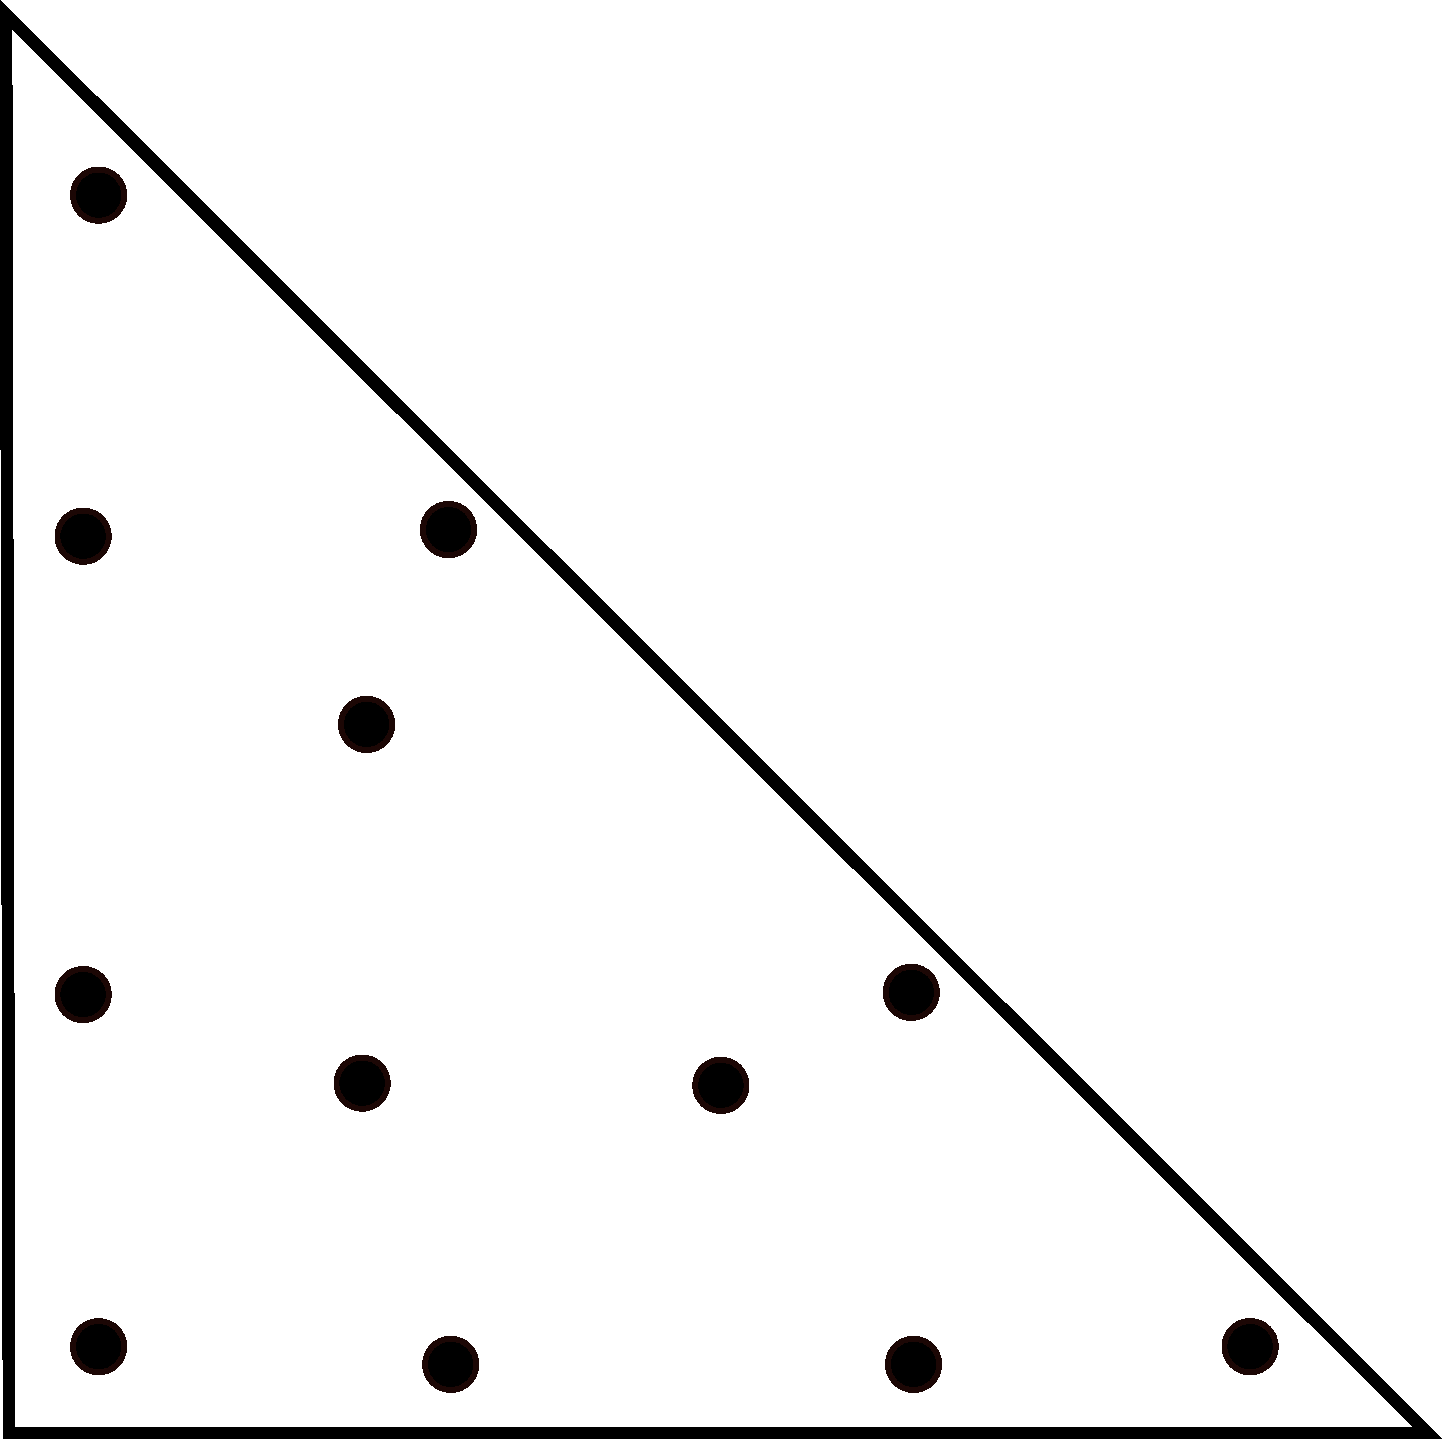
\includegraphics[scale=0.07]{image/quad_2d.pdf}
    \end{subfigure}
    \begin{subfigure}{0.45\textwidth}
      \centering
      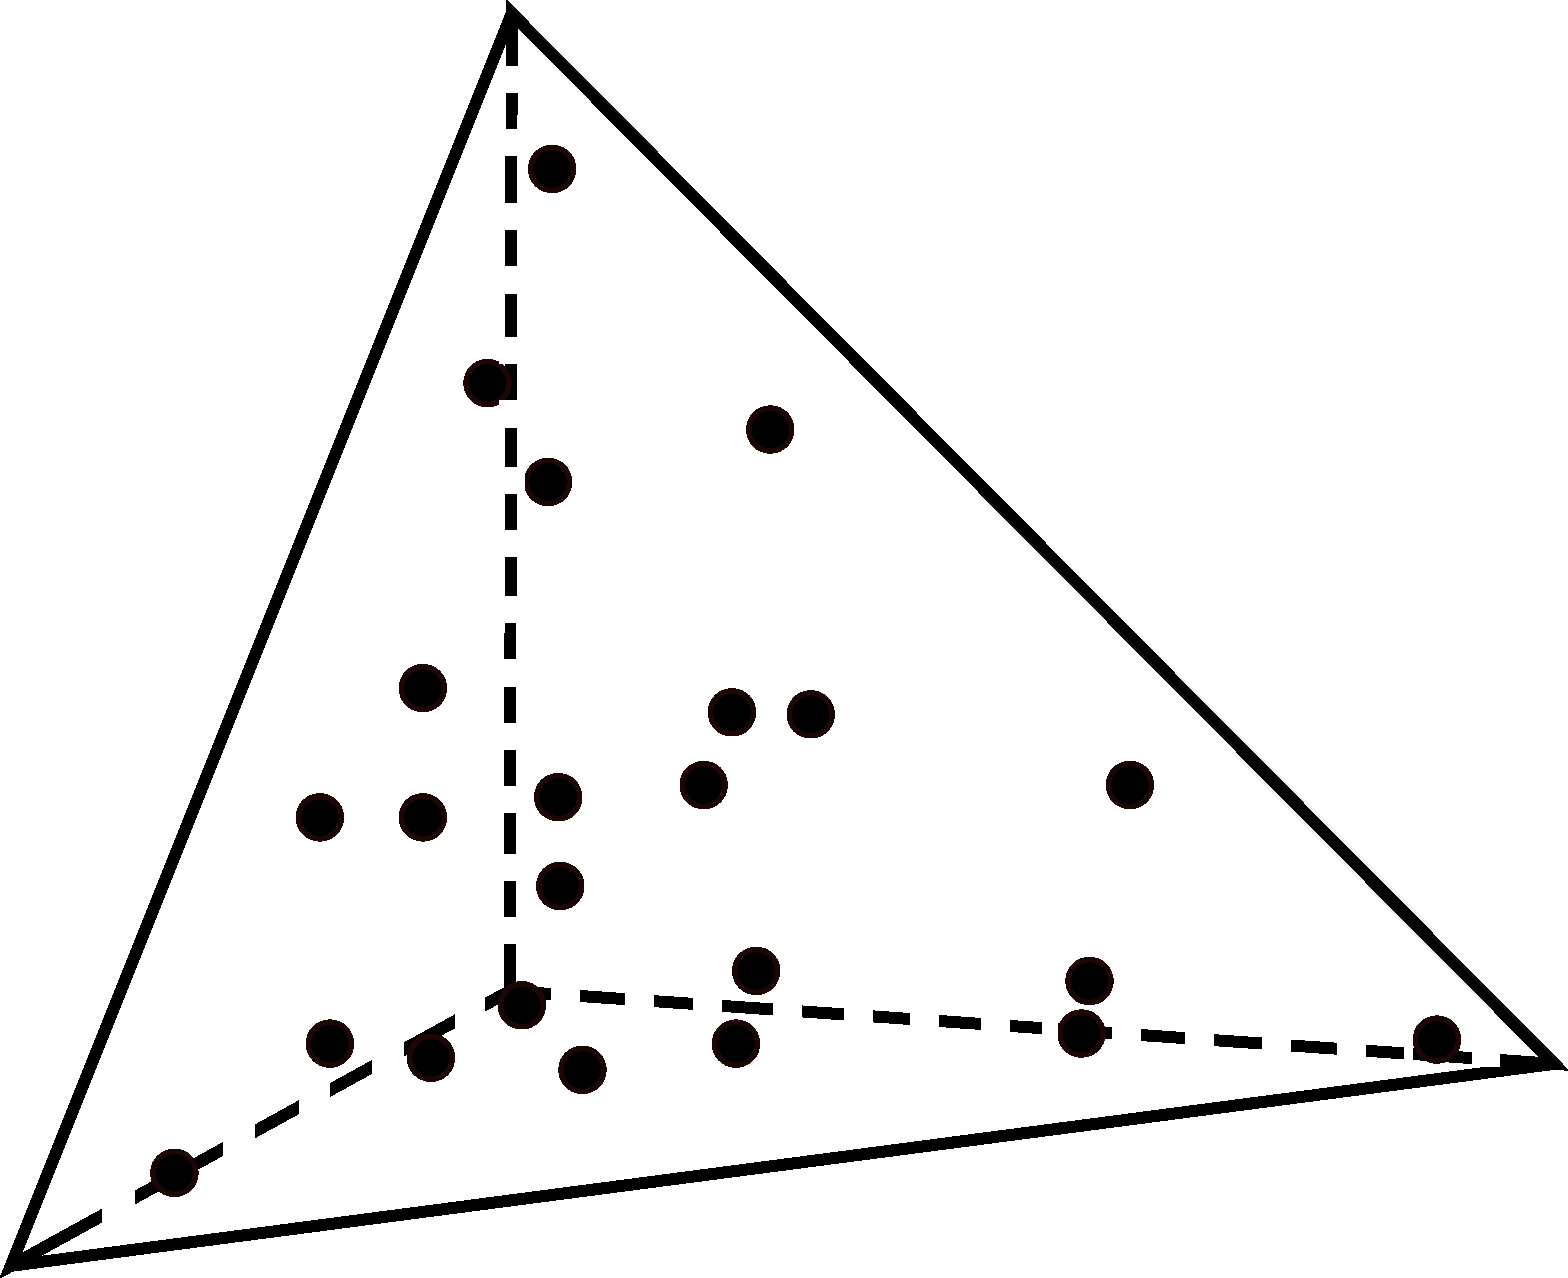
\includegraphics[scale=0.08]{image/quad_3d.pdf}
    \end{subfigure}
    \caption{\scriptsize{Quadrature points on 2D and 3D reference element for $\QuadOrder=6$.}}
    \label{quad_point_sketch}
  \end{figure}

  \uncover<2->{
  \begin{block}{\danger Warning}
    Such a parametrization requires enhanced output and visualization techniques.
  \end{block}
  }

\end{frame}


\begin{frame}{WADG small experiment}

  \setlength{\modelwidth}{6.0cm}
\begin{figure}[htbp]
\begin{subfigure}{1.0\textwidth}
  \renewcommand{\modelfile}{image/num_exp_1/bicouche_model}
     \renewcommand{\cmapmin}{1500}
     \renewcommand{\cmapmax}{3000}
     \centering
     \begin{tikzpicture}
\pgfmathsetmacro{\xmin} {0.}
\pgfmathsetmacro{\xmax} {9.7}
\pgfmathsetmacro{\zmin} {0.}
\pgfmathsetmacro{\zmax} {2.7}
\pgfmathsetmacro{\zzmax} {3.0}
\pgfmathsetmacro{\xxmax} {10.0}


\begin{axis}[%
width=1.0\modelwidth,
height=0.5\modelwidth,
axis on top, separate axis lines,
xmin=\xmin, xmax=\xxmax, %xlabel={x (km)},
ymin=\zmin, ymax=\zzmax,
yticklabels={},xticklabels={},
y dir=reverse,
colormap/paraview, colorbar,
colorbar style={title=\small{$m \cdot s^{-1}$}},
point meta min=\cmapmin, point meta max=\cmapmax,
colorbar/width=2.5mm,
axis x line=top,thick,
axis y line=left,thick,
ylabel style={rotate=-90},
ylabel={$z$},
xlabel={$x$},
ticks = none,
]
\addplot [forget plot] graphics [xmin=\xmin,xmax=\xmax,ymin=\zmin,ymax=\zmax] {{\modelfile}.png};
\end{axis}
\end{tikzpicture}%

     \caption{Bi-layered wavespeed model (reference).}
     \label{bicouche_model_with_mesh}
\end{subfigure}

\begin{subfigure}{0.45\textwidth}
  \renewcommand{\modelfile}{image/num_exp_1/bicouche_p4q1}
     \renewcommand{\cmapmin}{1500}
     \renewcommand{\cmapmax}{3000}
     \centering
     \begin{tikzpicture}
  \pgfmathsetmacro{\xmin} {0.}
\pgfmathsetmacro{\xmax} {9.7}
\pgfmathsetmacro{\zmin} {0.}
\pgfmathsetmacro{\zmax} {2.7}
\pgfmathsetmacro{\zzmax} {3.0}
\pgfmathsetmacro{\xxmax} {10.0}

\begin{axis}[%
width=1.0\modelwidth,
height=0.5\modelwidth,
axis on top, separate axis lines,
xmin=\xmin, xmax=\xxmax, %xlabel={x (km)},
ymin=\zmin, ymax=\zzmax,
yticklabels={},xticklabels={},
y dir=reverse,
point meta min=1.5e3, point meta max=5.5e3,
axis x line=top,thick,
axis y line=left,thick,
ylabel style={rotate=-90},
ylabel={$z$},
xlabel={$x$},
ticks = none,
]
\addplot [forget plot] graphics [xmin=\xmin,xmax=\xmax,ymin=\zmin,ymax=\zmax] {{\modelfile}.png};
\end{axis}
\end{tikzpicture}%

     \caption{Bi-layered wavespeed model (P4 Q1).}
     \label{bicouche_model_without_mesh}
\end{subfigure}
\hspace{0.5cm}
\begin{subfigure}{0.45\textwidth}
  \renewcommand{\modelfile}{image/num_exp_1/bicouche_p4q9}
     \renewcommand{\cmapmin}{1500}
     \renewcommand{\cmapmax}{3000}
     \centering
     \begin{tikzpicture}
  \pgfmathsetmacro{\xmin} {0.}
\pgfmathsetmacro{\xmax} {9.7}
\pgfmathsetmacro{\zmin} {0.}
\pgfmathsetmacro{\zmax} {2.7}
\pgfmathsetmacro{\zzmax} {3.0}
\pgfmathsetmacro{\xxmax} {10.0}

\begin{axis}[%
width=1.0\modelwidth,
height=0.5\modelwidth,
axis on top, separate axis lines,
xmin=\xmin, xmax=\xxmax, %xlabel={x (km)},
ymin=\zmin, ymax=\zzmax,
yticklabels={},xticklabels={},
y dir=reverse,
point meta min=1.5e3, point meta max=5.5e3,
axis x line=top,thick,
axis y line=left,thick,
ylabel style={rotate=-90},
ylabel={$z$},
xlabel={$x$},
ticks = none,
]
\addplot [forget plot] graphics [xmin=\xmin,xmax=\xmax,ymin=\zmin,ymax=\zmax] {{\modelfile}.png};
\end{axis}
\end{tikzpicture}%

     \caption{Bi-layered wavespeed model (P4 Q9).}
     \label{bicouche_model_with_wadg}
\end{subfigure}
\caption{Illustration of the wavespeed model for three different configurations.}
\label{bicouche_meshes}
\end{figure}
\end{frame}


\begin{frame}{WADG small experiment}
\vspace{-0.3cm}
\begin{figure}[htbp]
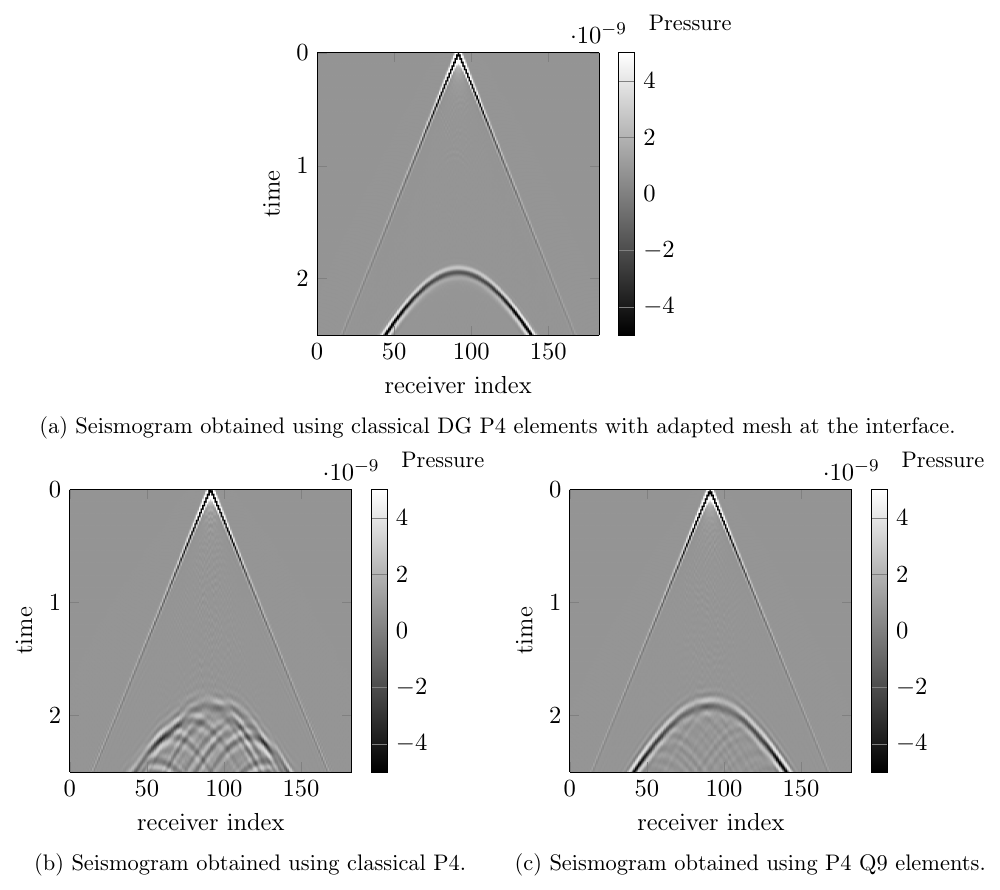
\includegraphics[scale=0.25]{image/flemme_wadg.png}
\end{figure}


\end{frame}



\begin{frame}{Computational cost of WADG (2D)}
\colorlet{xcolorA}{red!80!black}
\colorlet{xcolorB}{red!60!black}
\colorlet{ycolorA}{blue!80!black}
\colorlet{ycolorB}{blue!60!black}


\begin{figure}[H]
\centering
\begin{tikzpicture}[scale=0.7]
  \pgfplotsset{ybar stacked, ymin=0, ymax=200, xmin=1.5, xmax=5.5, xtick=data, xlabel=$\PolOrder$, ylabel=\% of CPU time,
  }
  \begin{axis}[bar shift=-8pt,
    legend pos = outer north east, legend style = {name = serieA},
    ylabel]
    \addplot [draw=ycolorA, pattern= north west lines, pattern color=ycolorA] table [x index = 0, y index = 1] {./graph/num_exp_1/serieA.dat};
    \addplot [draw=blue, pattern=horizontal lines light blue] table [x index = 0, y index = 2] {./graph/num_exp_1/serieA.dat};
    \legend{RHS CPU time (WADG), Apply model CPU time (WADG)}
    \legend{Surface + Volume ($\QuadOrder = 1$), Apply model ($\QuadOrder = 1$)}
  \end{axis}
  \begin{axis}[bar shift = 8pt,
    legend style = {at = {([yshift = -3.5mm, xshift = -3.7mm]serieA.south west)},
      anchor = north west}]
    \addplot [pattern color=ycolorB, pattern=north east lines] table [x index = 0, y index = 1] {./graph/num_exp_1/serieB.dat};
    \addplot [draw=xcolorB, pattern=dots, pattern color=xcolorB] table [x index = 0, y index = 2] {./graph/num_exp_1/serieB.dat};
    \legend{Surface + Volume ($\QuadOrder = 2\PolOrder+1$), Apply model ($\QuadOrder = 2\PolOrder+1$)}
  \end{axis}
\end{tikzpicture}
\caption{Histogram illustrating the computational proportion of the model operators in
the time derivative evaluation in 2D.}
\label{histo_wadg}
\end{figure}

\end{frame}



\begin{frame}{Computational cost of WADG (3D)}
\colorlet{xcolorA}{red!80!black}
\colorlet{xcolorB}{red!60!black}
\colorlet{ycolorA}{blue!80!black}
\colorlet{ycolorB}{blue!60!black}


\begin{figure}[H]
\centering
\begin{tikzpicture}[scale=0.7]
  \pgfplotsset{ybar stacked, ymin=0, ymax=180, xmin=1.5, xmax=4.5, xtick=data, xlabel=$\PolOrder$, ylabel=\% of CPU time,
  }
  \begin{axis}[bar shift=-8pt,
    legend pos = outer north east, legend style = {name = serieA},
    ylabel]
    \addplot [draw=ycolorA, pattern= north west lines, pattern color=ycolorA] table [x index = 0, y index = 1] {./graph/num_exp_1/serieA_3D.dat};
    \addplot [draw=blue, pattern=horizontal lines light blue] table [x index = 0, y index = 2] {./graph/num_exp_1/serieA_3D.dat};
    \legend{RHS CPU time (WADG), Apply model CPU time (WADG)}
    \legend{Surface + Volume ($\QuadOrder = 1$), Apply model ($\QuadOrder = 1$)}
  \end{axis}
  \begin{axis}[bar shift = 8pt,
    legend style = {at = {([yshift = -3.5mm,xshift = -3.7mm]serieA.south west)},
      anchor = north west}]
    \addplot [pattern color=ycolorB, pattern=north east lines] table [x index = 0, y index = 1] {./graph/num_exp_1/serieB_3D.dat};
    \addplot [draw=xcolorB, pattern=dots, pattern color=xcolorB] table [x index = 0, y index = 2] {./graph/num_exp_1/serieB_3D.dat};
    \legend{Surface + Volume ($\QuadOrder = 2\PolOrder+1$), Apply model ($\QuadOrder = 2\PolOrder+1$)}
  \end{axis}
\end{tikzpicture}
\caption{Histogram illustrating the computational proportion of the model operators in
the time derivative evaluation in 3D.}
\label{histo_wadg_3D}
\end{figure}
\end{frame}
